\chapter{Release 1}

\newpage

%============================================================
\section{Introduction}
%============================================================

Ce chapitre est essentiel pour le déroulement du projet, puisqu'il présente en détail la première version du produit final, appelée Release~1. La sortie de cette version est très importante car elle rassemble les fonctionnalités essentielles de notre projet et est indispensable pour finaliser la deuxième partie des fonctionnalités.

%============================================================
\section{Sprint 1 : Gestion des Accès et Administration des Comptes}
%============================================================

Ce sprint a pour objectif de développer le module d'authentification et de gestion des comptes utilisateurs, ainsi que la réinitialisation de mot de passe, permettant un accès sécurisé à la plateforme selon les rôles définis (Administrateur, Responsable RH et Employé).

\subsection{Objectif du sprint 1}

L'objectif de ce sprint est d'implémenter l'authentification du système, la gestion des comptes (Administrateur, Responsable RH, Employé) et le contrôle d'accès sécurisé à la plateforme.

\subsection{Durée du sprint 1}

\begin{itemize}
    \item \textbf{Date de début du sprint} : 14/02/2026
    \item \textbf{Date de fin du sprint} : 11/03/2026
\end{itemize}

\subsection{Backlog du sprint 1}
Ce tableau présente les neuf user stories retenues pour le sprint 1, couvrant la gestion des comptes Administrateur, Responsable RH et Employé, ainsi que l'authentification et la réinitialisation du mot de passe. Chaque user story est accompagnée de sa priorité (P) et de sa complexité estimée (C).

sprint. Le sprint backlog du sprint 1 est présenté dans le tableau suivant :

\begin{longtable}{|>{\centering\arraybackslash}m{0.5cm}|
    >{\centering\arraybackslash}m{3cm}|
    >{\centering\arraybackslash}m{2.5cm}|
    >{\centering\arraybackslash}m{3cm}|
    >{\centering\arraybackslash}m{3cm}|
    >{\centering\arraybackslash}m{0.7cm}|
    >{\centering\arraybackslash}m{0.9cm}|}
\hline
\textbf{ID} & \textbf{User Story} & \textbf{En tant que} & \textbf{Je veux} & \textbf{Afin de} & \textbf{P} & \textbf{C} \\
\hline
\endfirsthead
\hline
\textbf{ID} & \textbf{User Story} & \textbf{En tant que} & \textbf{Je veux} & \textbf{Afin de} & \textbf{P} & \textbf{C} \\
\hline
\endhead
1  & Créer compte responsable RH    & Administrateur  & créer un compte responsable RH    & administrer la plateforme        & 5 & 2 \\ \hline
2  & Modifier compte responsable RH & Administrateur  & modifier un compte responsable RH & administrer la plateforme        & 4 & 2 \\ \hline
3  & Supprimer compte responsable RH& Administrateur  & supprimer un compte responsable RH& administrer la plateforme        & 4 & 2 \\ \hline
5  & S'inscrire                     & Responsable RH  & créer mon compte sur la plateforme& accéder au système de gestion RH & 5 & 2 \\ \hline
7  & Créer compte employé           & Responsable RH  & créer un compte employé           & permettre l'accès au système     & 5 & 2 \\ \hline
8  & Modifier compte employé        & Responsable RH  & modifier un compte employé        & mettre à jour les données        & 4 & 2 \\ \hline
9  & Supprimer compte employé       & Responsable RH  & supprimer un compte employé       & désactiver l'accès               & 4 & 2 \\ \hline
31 & S'authentifier                 & Employé + Responsable RH + Administrateur & me connecter et me déconnecter    & accéder à mon espace sécurisé    & 5 & 2 \\ \hline

\caption{Backlog Sprint 1 — Accès \& Identités}
\end{longtable}


\subsection{Spécification fonctionnelle détaillée}

\subsubsection*{Diagramme de cas d'utilisation du sprint 1}

Ce diagramme illustre les interactions entre les trois acteurs principaux — Administrateur, Responsable RH et Employé — et les fonctionnalités du sprint 1, notamment la gestion des comptes et l'authentification.
\begin{figure}[H]
    \centering
    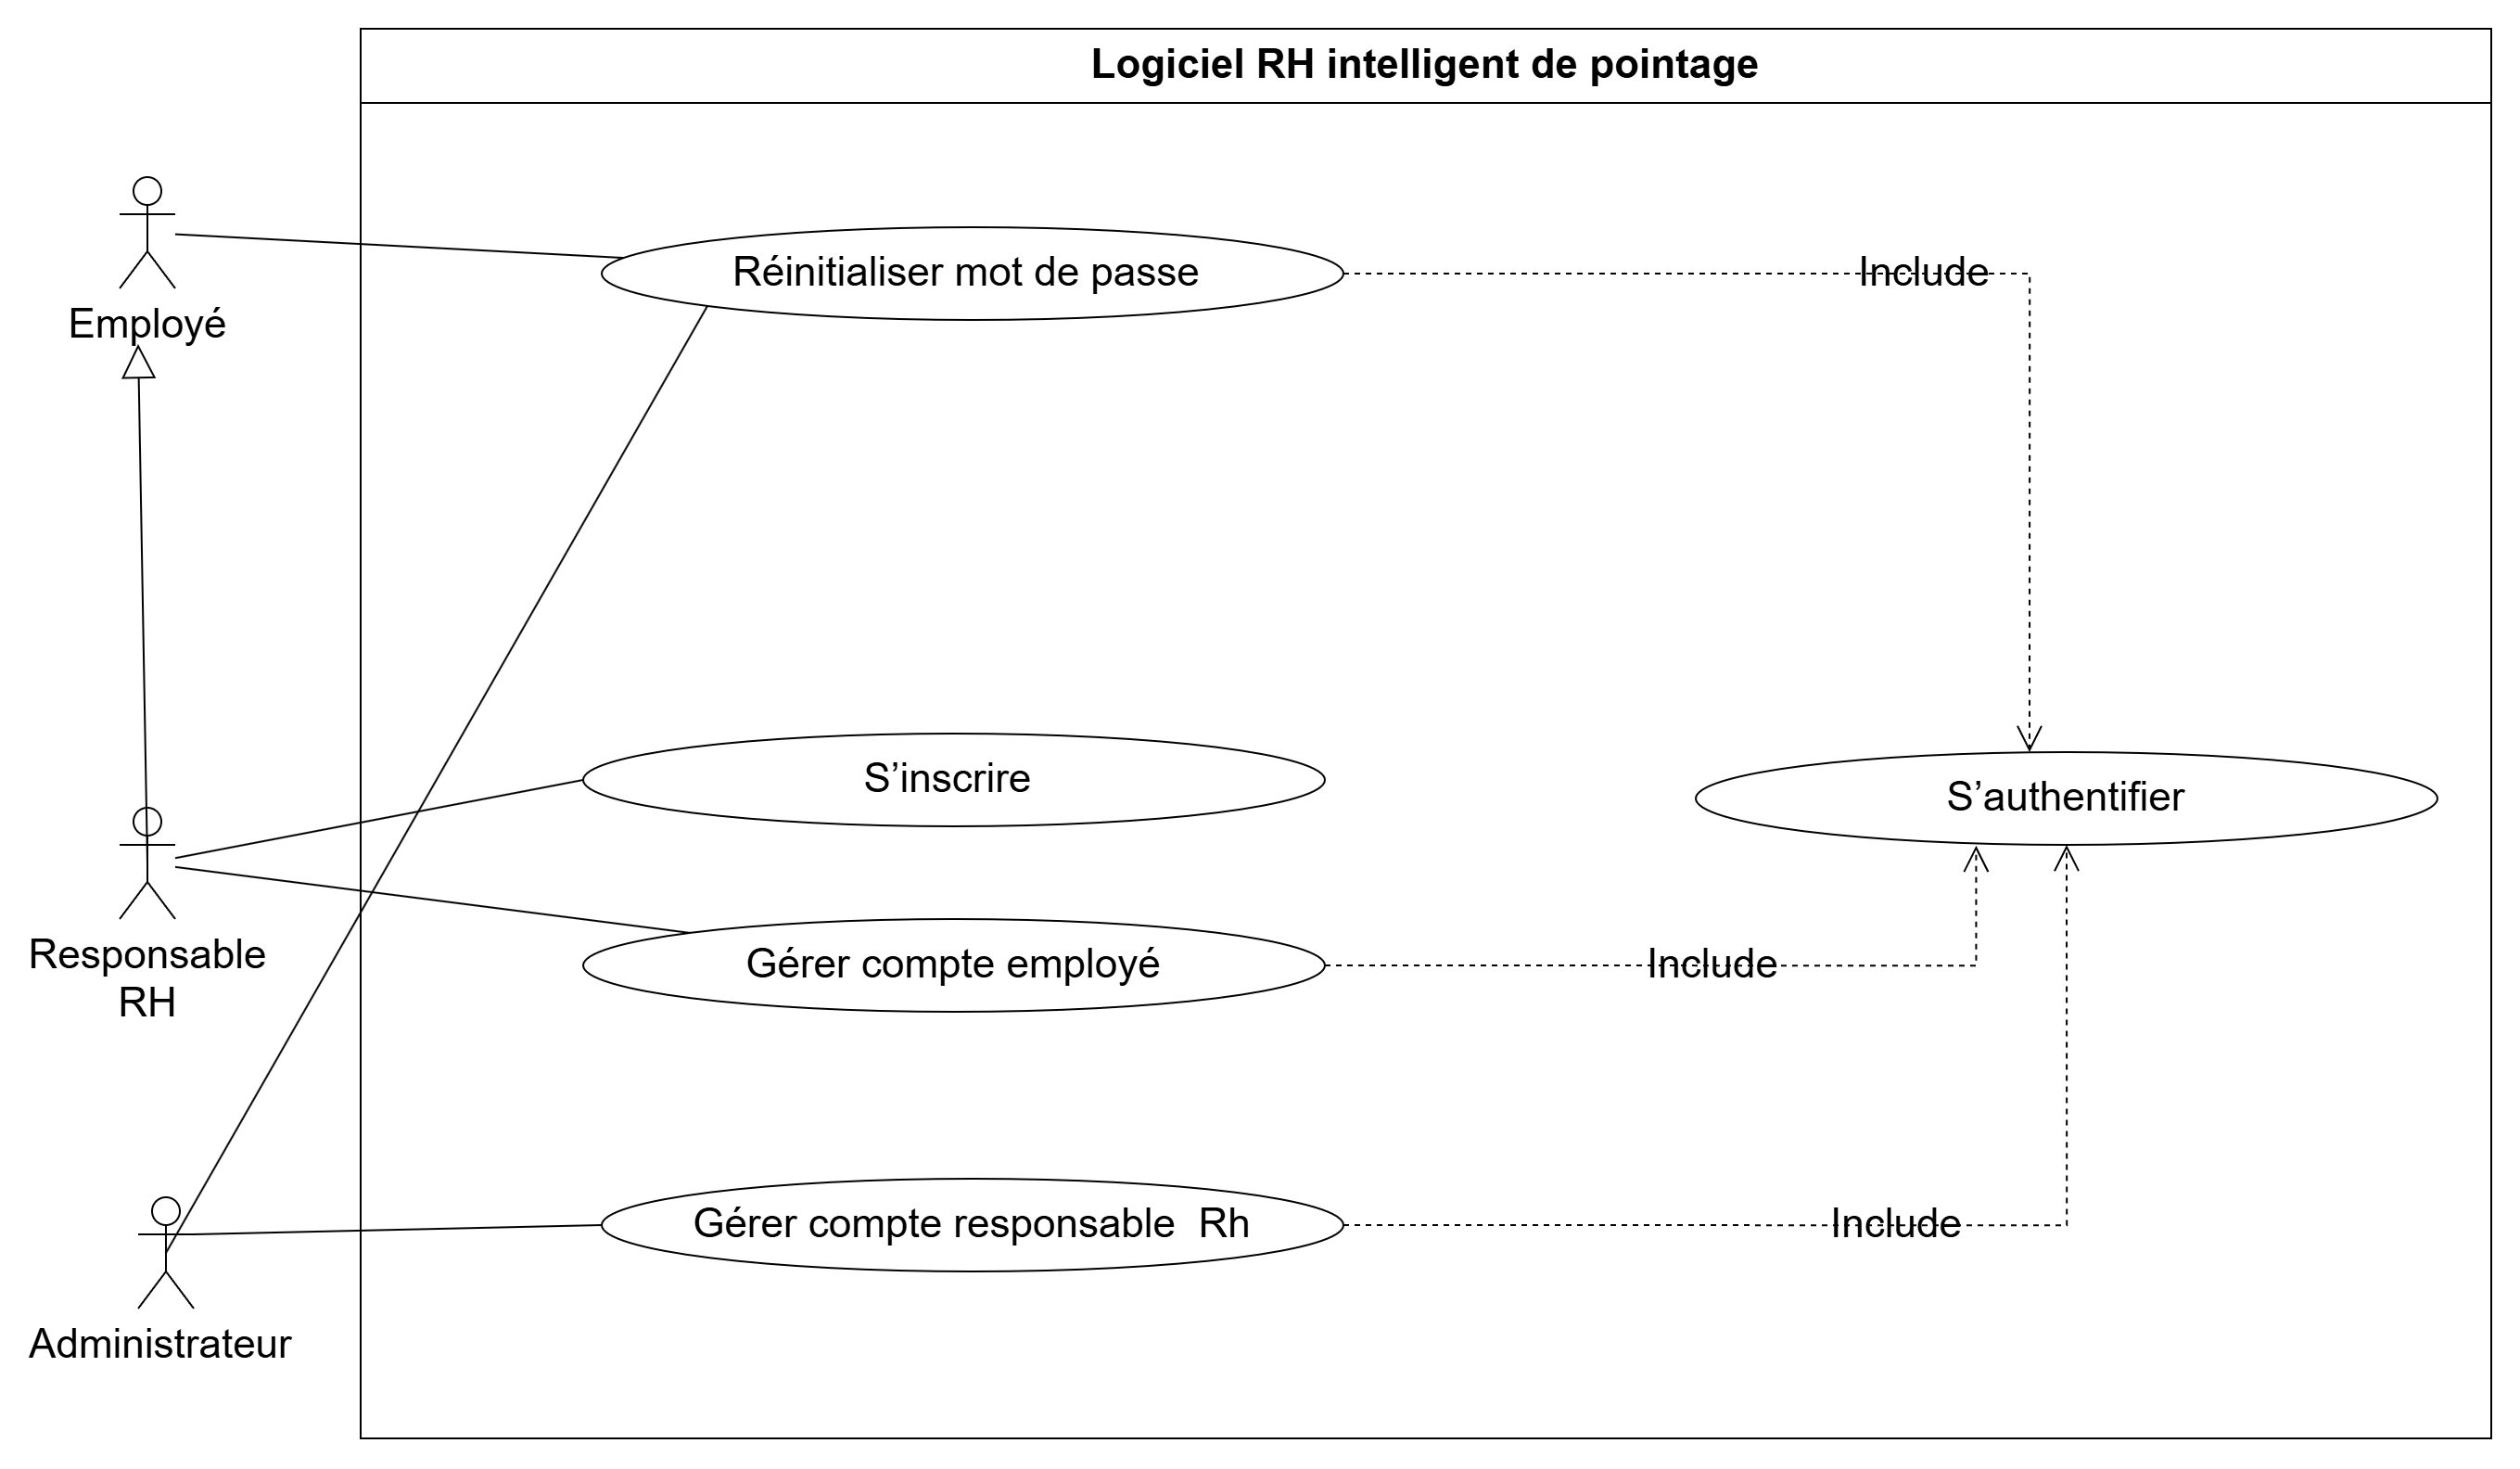
\includegraphics[width=0.9\textwidth]{projet/images/usecase/sprint1/use_case_sprint1.png}
    \caption{Diagramme de Cas d'utilisation du Sprint 1}
    \label{fig:usecase1}
\end{figure}







\subsubsection*{Description textuelle : cas d'utilisation « S'authentifier »}
Ce tableau présente le scénario d'authentification d'un utilisateur, depuis l'accès à la page de connexion jusqu'à la redirection vers le tableau de bord, ainsi que le cas d'exception lié à des identifiants invalides.
\begin{longtable}{|p{5cm}|p{11cm}|}
\hline
\textbf{Nom du cas d'utilisation} & \textbf{S'authentifier} \\ \hline
\textbf{Acteurs}                  & Utilisateur \\ \hline
\textbf{Objectif}                 & Permettre à l'utilisateur d'accéder au système \\ \hline
\textbf{Préconditions}            & L'utilisateur possède un compte valide \\ \hline
\textbf{Scénario nominal} &
1. L'utilisateur accède à la page de connexion. \newline
2. Le système affiche le formulaire de connexion . \newline
3. L'utilisateur saisit son login et son mot de passe  \newline
4. L'utilisateur clique sur « Se connecter ». \newline
5. Le système envoie les identifiants pour vérification. \newline
6. Le système valide les identifiants. \newline
7. Le système affiche le tableau de bord. \newline
8. L'utilisateur est redirigé avec succès. \\ \hline
\textbf{Scénario d'exception} &
1.1 Si les identifiants sont invalides : \newline
Le système affiche un message d'erreur. \\ \hline
\textbf{Post-condition} & L'utilisateur est connecté et accède à son tableau de bord \\ \hline
\caption{Description textuelle du cas d'utilisation « S'authentifier »}
\end{longtable}



\subsubsection*{Description textuelle : cas d'utilisation « S'inscrire »}
Ce tableau détaille le processus d'inscription d'un nouveau Responsable RH, en présentant les étapes de saisie des informations, de vérification par le système et de création du compte, ainsi que le scénario d'exception en cas d'échec.

\begin{longtable}{|p{5cm}|p{11cm}|}
\hline
\textbf{Nom du cas d'utilisation} & \textbf{S'inscrire} \\ \hline
\textbf{Acteurs}                  & Responsable RH \\ \hline
\textbf{Objectif}                 & Permettre à un nouvel utilisateur de créer un compte sur la plateforme \\ \hline
\textbf{Préconditions}            & L'utilisateur ne possède pas encore de compte \\ \hline
\textbf{Scénario nominal} &
1. L'utilisateur accède à la page d'inscription. \newline
2. L'utilisateur saisit les informations demandées . \newline
3. Le système vérifie les informations reçues. \newline
4. Le système enregistre les informations dans la base de données. \newline
5. L'utilisateur est redirigé vers son tableau de bord. \\ \hline
\textbf{Scénario d'exception} &
5.1 Si les informations sont invalides ou l'inscription échoue, le système affiche un message d'erreur et demande de réessayer. \\ \hline
\textbf{Post-condition} & Un nouveau compte utilisateur est créé et l'utilisateur peut accéder à la plateforme. \\ \hline
\caption{Description textuelle du cas d'utilisation « S'inscrire »}
\end{longtable}


\subsubsection*{Raffinement du cas d'utilisation « Gérer compte employé »}
Ce diagramme raffine le cas d'utilisation « Gérer compte employé » en décomposant les trois opérations possibles : la création, la modification et la suppression d'un compte employé par le Responsable RH.

\begin{figure}[H]
    \centering
    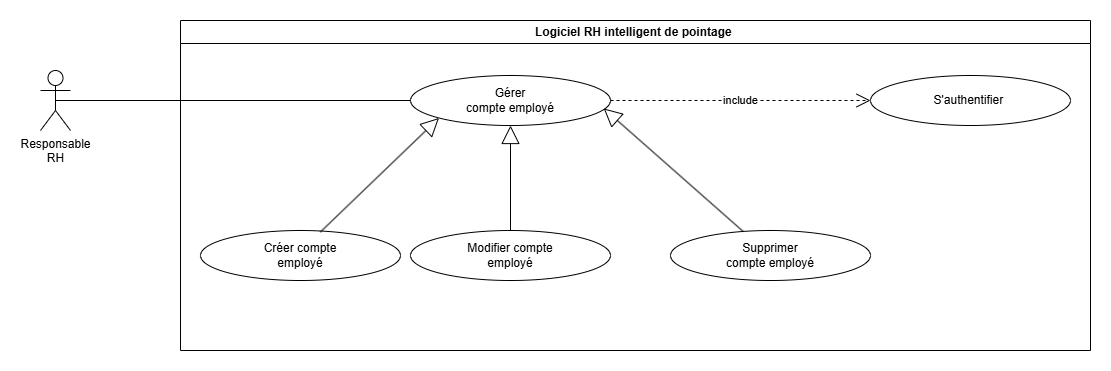
\includegraphics[width=0.9\textwidth]{projet/images/usecase/sprint1/gerer_compte_employe.png}
    \caption{Raffinement du cas d'utilisation « Gérer compte employé »}
    \label{fig:usecase2}
\end{figure}


\subsubsection*{Description textuelle : cas d'utilisation « Gérer compte employé »}
Ce tableau décrit les scénarios de création, modification et suppression d'un compte employé, incluant le processus d'envoi d'un lien d'activation par e-mail et les exceptions liées à des données invalides.

\begin{longtable}{|p{5cm}|p{11cm}|}
\hline
\textbf{Nom du cas d'utilisation} & \textbf{Gérer compte employé} \\ \hline
\textbf{Acteurs}                  & Responsable RH \\ \hline
\textbf{Objectif}                 & Créer, modifier et supprimer un compte employé \\ \hline
\textbf{Préconditions}            & Responsable RH authentifié et compte employé existant ou en cours de création \\ \hline
\textbf{Scénario nominal} &
\textbf{Création :} \newline
1. Le Responsable RH accède à la gestion des employés. \newline
2. Il clique sur « Ajouter employé ». \newline
3. Il saisit les informations de l'employé. \newline
4. Il valide la création. \newline
5. Le système crée le compte. \newline
6. Le système envoie un email contenant un lien de définition du mot de passe. \newline
7. L'employé clique sur le lien reçu par email. \newline
8. Il définit son mot de passe pour activer son compte. \newline
\textbf{Modification :} \newline
9. Le Responsable RH accède à la liste des employés. \newline
10. Il sélectionne un employé. \newline
11. Il clique sur « Modifier compte ». \newline
12. Le Responsable RH fait des modifications. \newline
13. Le système met à jour le compte. \newline
\textbf{Suppression :} \newline
14. Le Responsable RH accède à la liste des employés. \newline
15. Il sélectionne un employé. \newline
16. Il clique sur « Supprimer compte ». \newline
17. Le système supprime le compte de l'employé. \\ \hline
\textbf{Scénario d'exception} &
3.1 Si les données sont invalides, le système affiche une erreur. \newline
12.1 Si les données modifiées sont invalides, le système affiche une erreur. \\ \hline
\textbf{Post-condition} & Le compte employé est créé, modifié ou supprimé selon l'action effectuée. \\ \hline
\caption{Description textuelle du cas d'utilisation « Gérer compte employé »}
\end{longtable}


\subsubsection*{Raffinement du cas d'utilisation « Gérer compte Responsable RH »}
Ce diagramme raffine le cas d'utilisation « Gérer compte Responsable RH » en illustrant les actions de création, modification et suppression d'un compte Responsable RH effectuées par l'Administrateur.

\begin{figure}[H]
    \centering
    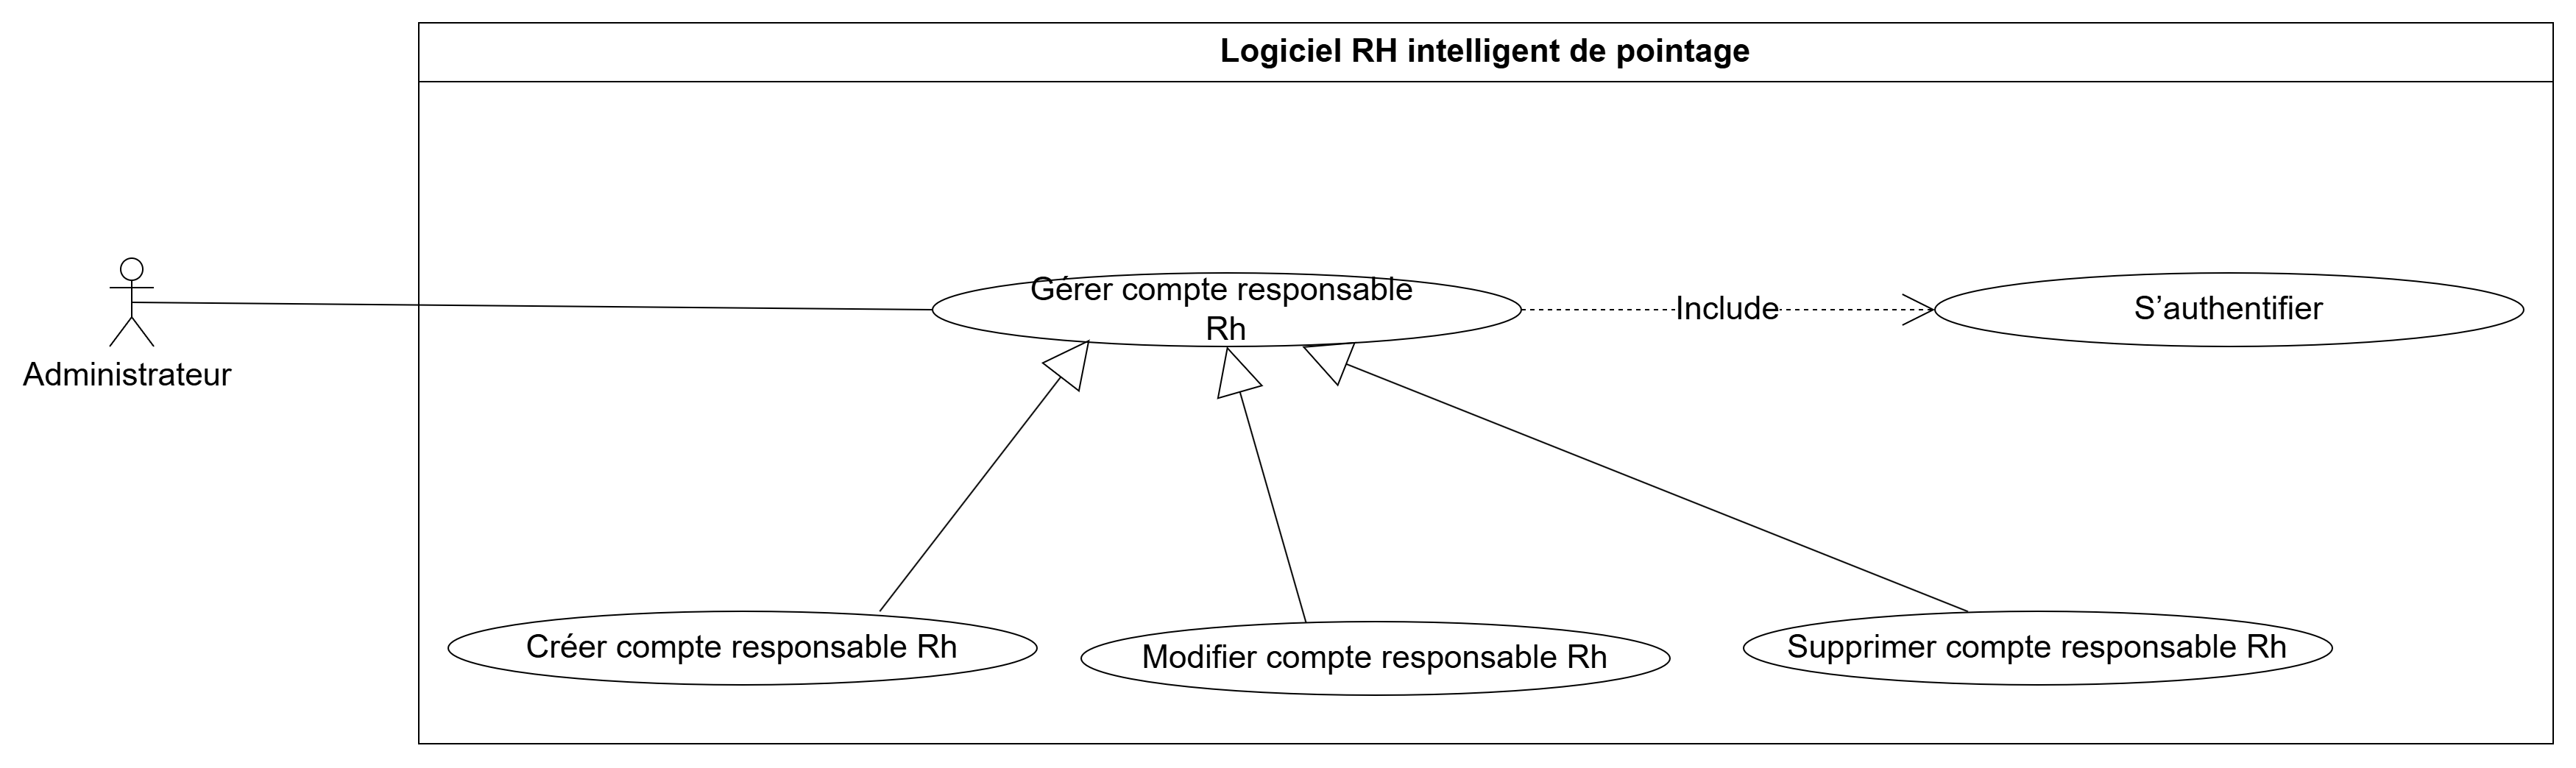
\includegraphics[width=0.9\textwidth]{projet/images/usecase/sprint1/gere_compte_rh.png}
    \caption{Raffinement du cas d'utilisation « Gérer compte Responsable RH »}
    \label{fig:usecase3}
\end{figure}


\subsubsection*{Description textuelle : cas d'utilisation « Gérer compte Responsable RH »}
Ce tableau présente les étapes détaillées de gestion d'un compte Responsable RH par l'Administrateur, avec les scénarios d'exception associés, notamment la vérification des doublons lors de la création et la demande de confirmation avant suppression.

\begin{longtable}{|p{5cm}|p{11cm}|}
\hline
\textbf{Nom du cas d'utilisation} & \textbf{Gérer compte Responsable RH} \\ \hline
\textbf{Acteurs}                  & Administrateur \\ \hline
\textbf{Objectif}                 & Créer, modifier et supprimer un compte Responsable RH \\ \hline
\textbf{Préconditions}            & L'administrateur doit être authentifié \\ \hline
\textbf{Scénario nominal} &
\textbf{Création :} \newline
1. L'administrateur accède à l'interface de gestion utilisateur. \newline
2. L'administrateur clique sur « Ajouter un compte RH ». \newline
3. L'administrateur saisit les informations nécessaires (nom, nom entreprise, email, mot de passe). \newline
4. L'administrateur valide la création. \newline
5. Le système enregistre et crée le compte. \newline
\textbf{Modification :} \newline
6. L'administrateur accède à la liste des comptes. \newline
7. L'administrateur sélectionne un compte Responsable RH. \newline
8. L'administrateur modifie les informations. \newline
9. L'administrateur valide les modifications. \newline
10. Le système met à jour le compte. \newline
\textbf{Suppression :} \newline
11. L'administrateur sélectionne un compte. \newline
12. L'administrateur clique sur « Supprimer ». \newline
13. Le système demande confirmation. \newline
14. L'administrateur confirme. \newline
15. Le système supprime le compte. \\ \hline
\textbf{Scénario d'exception} &
3.1 Si des champs sont vides ou invalides, le système affiche un message d'erreur. \newline
5.1 Si le compte existe déjà, le système refuse la création. \newline
8.1 Si les informations modifiées sont invalides, le système affiche un message. \newline
14.1 Si l'administrateur annule, aucune suppression n'est effectuée. \\ \hline
\textbf{Post-condition} & Le compte est créé, modifié ou supprimé selon l'action effectuée. \\ \hline
\caption{Description textuelle du cas d'utilisation « Gérer compte Responsable RH »}
\end{longtable}


%============================================================
\subsection{Conception}
%============================================================

Cette section présente les différents diagrammes UML réalisés afin de modéliser le fonctionnement du système, notamment les diagrammes de séquence et les diagrammes de classes, permettant de décrire les interactions entre les acteurs ainsi que la structure globale de l'application.

\subsubsection{Diagrammes de séquence du sprint 1}

\subsubsection*{Diagramme de séquence du cas d'utilisation « S'authentifier »}

Ce diagramme représente le processus d'authentification d'un utilisateur sur la plateforme. L'utilisateur entre ses coordonnées, le système vérifie si ceux-ci sont valides et lui accorde ou refuse l'accès à son espace personnel.

\begin{figure}[H]
    \centering
    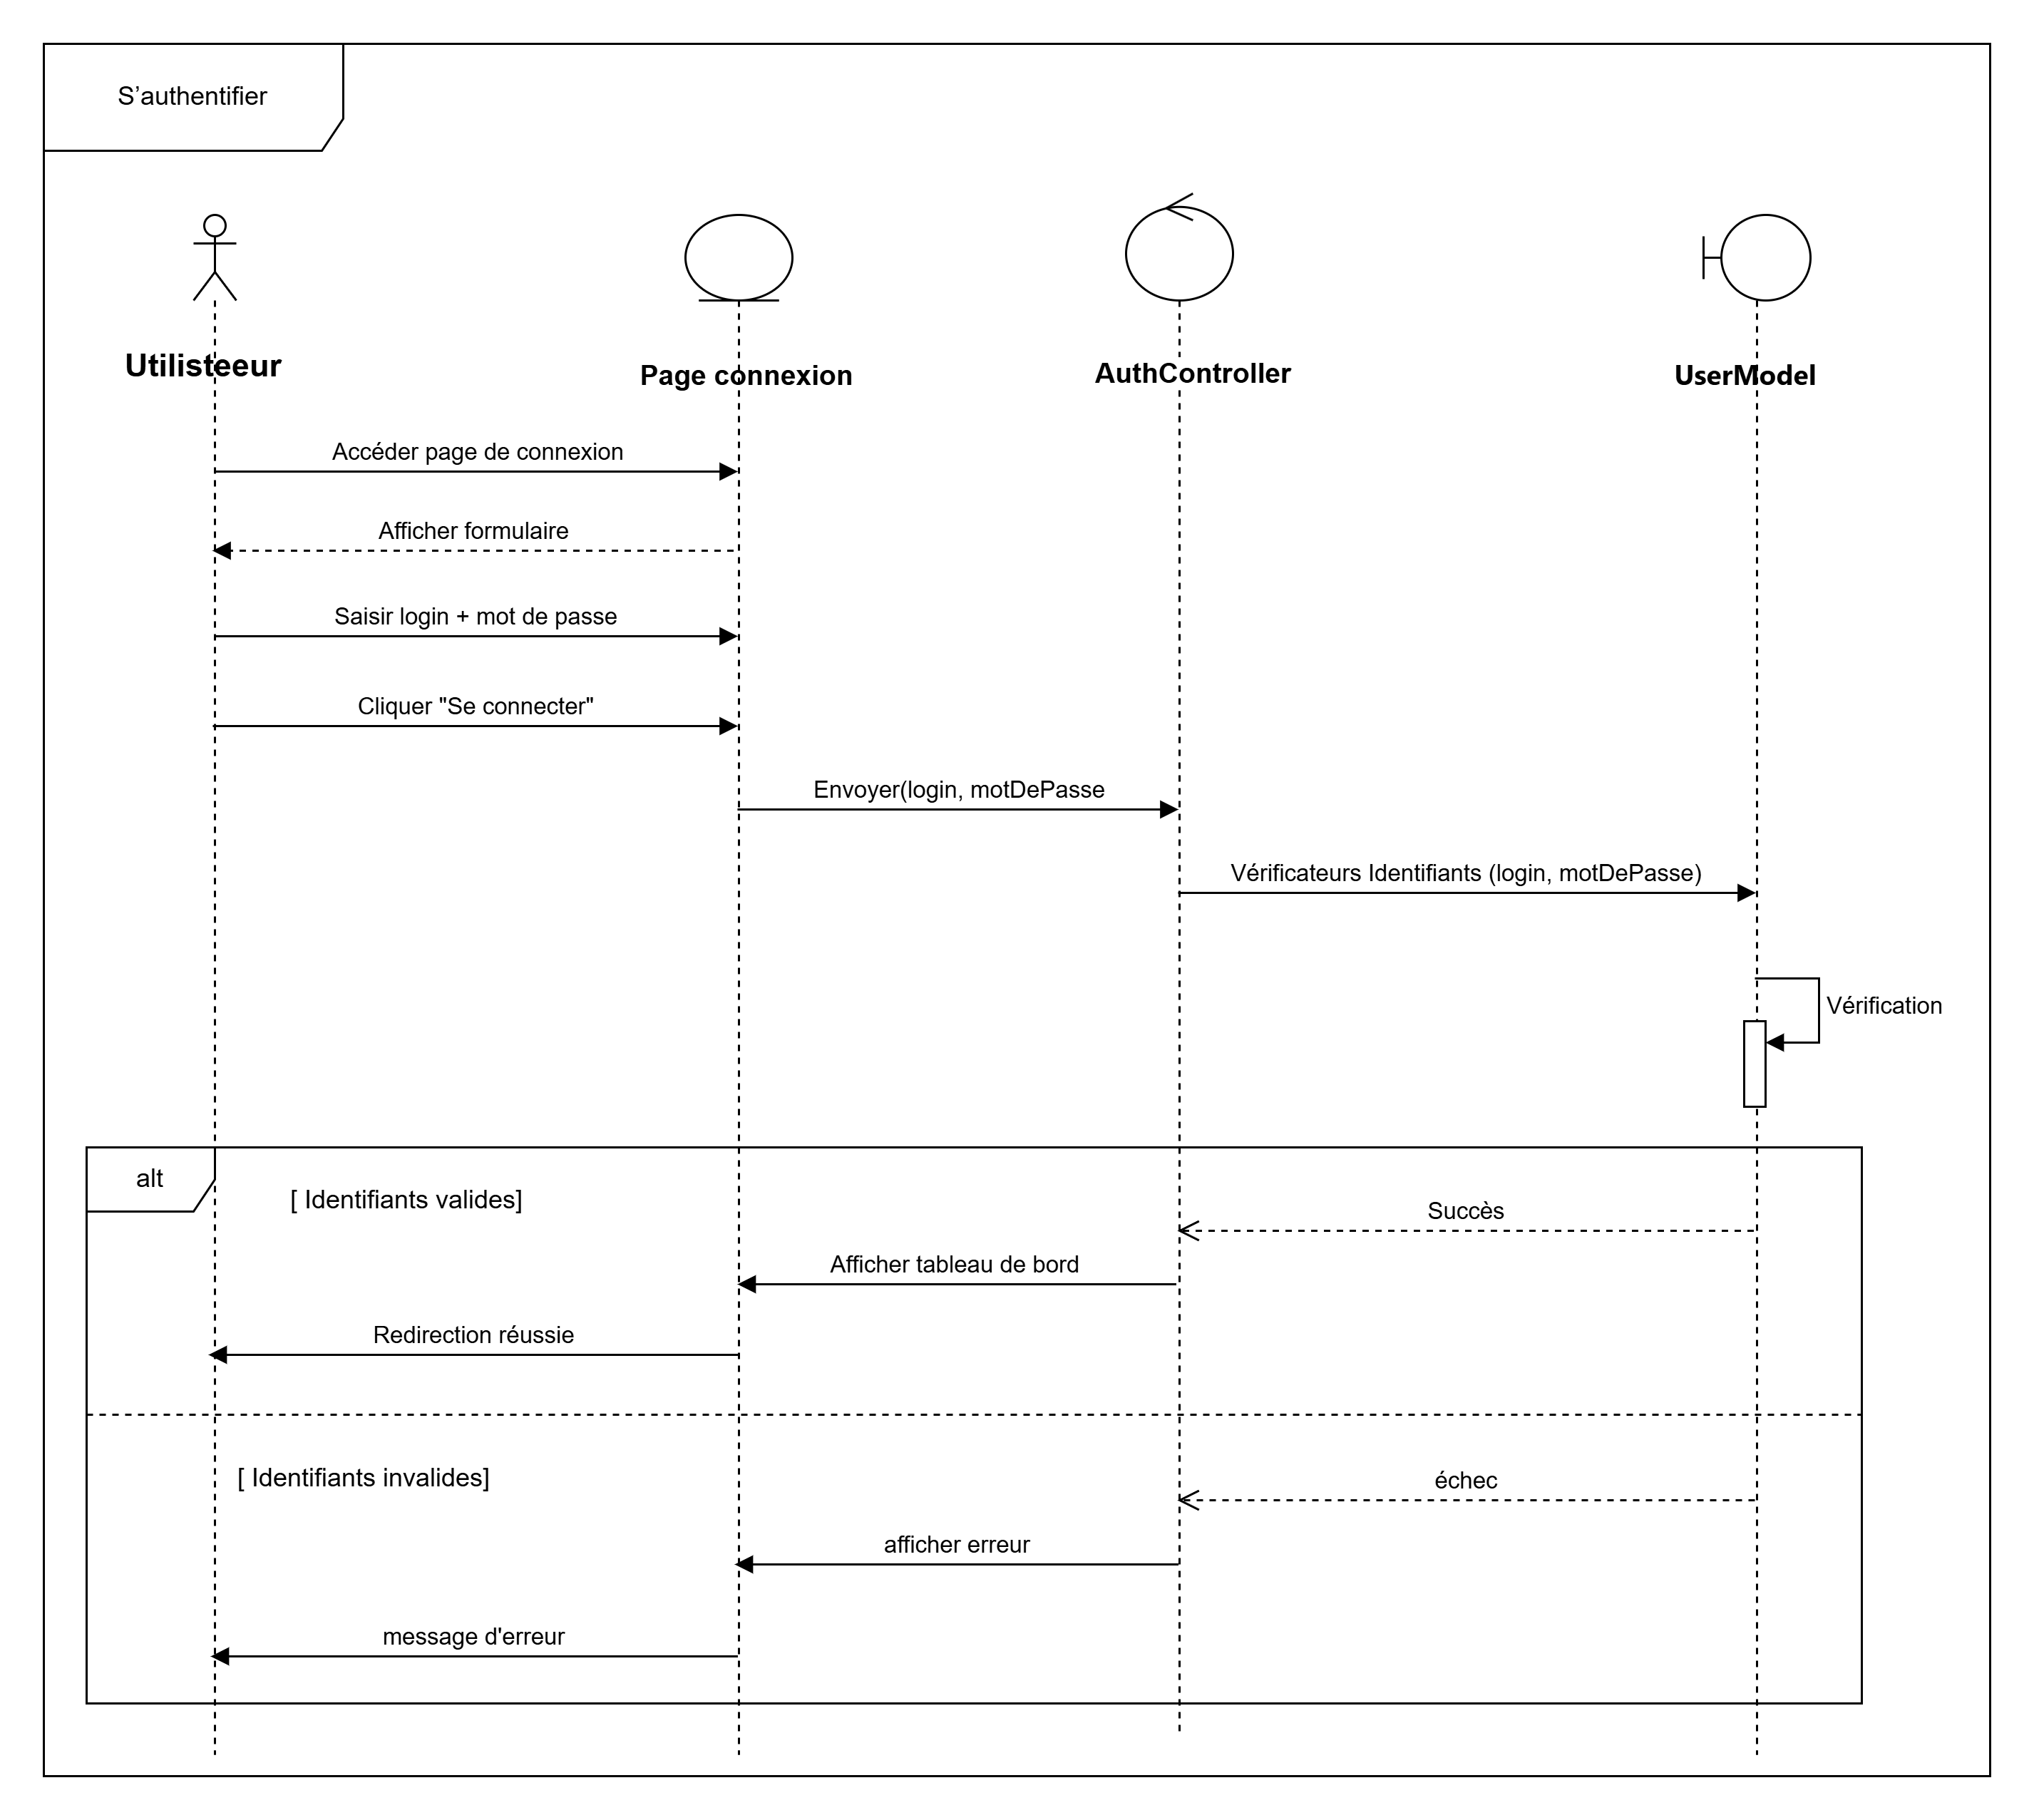
\includegraphics[width=0.9\textwidth]{projet/images/img sequence s1/auth.drawio.png}
    \caption{Diagramme de séquence du cas d'utilisation « S'authentifier »}
    \label{fig:interface6}
\end{figure}




Ce diagramme illustre les interactions entre l'utilisateur et le système lors de la réinitialisation du mot de passe, depuis la soumission de la demande jusqu'à la génération et l'envoi du nouveau mot de passe par e-mail.

\subsubsection*{Diagramme de séquence du cas d'utilisation « S'inscrire »}

Ce diagramme présente le processus d'inscription d'un nouveau Responsable RH sur la plateforme. Il saisit ses informations, le système vérifie leur validité, crée le compte et le redirige vers son tableau de bord.

\begin{figure}[H]
    \centering
    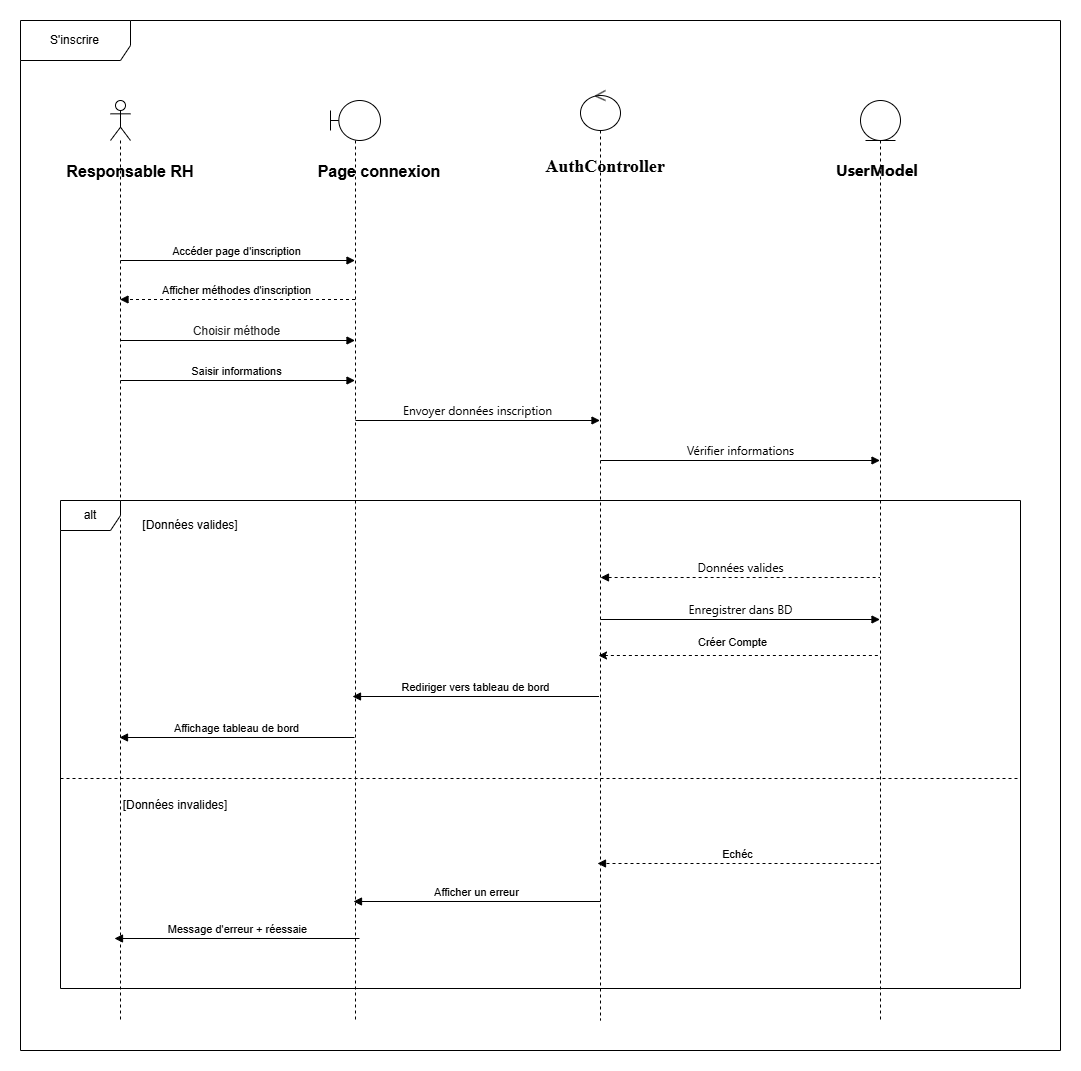
\includegraphics[width=0.9\textwidth]{projet/images/img sequence s1/sinscrire.drawio.png}
    \caption{Diagramme de séquence du cas d'utilisation « S'inscrire »}
\end{figure}


\subsubsection*{Diagramme de séquence du cas d'utilisation « Créer compte employé »}

Ce diagramme démontre la création d'un compte par le Responsable RH. Il entre les données de l'employé, puis le système valide ces informations et enregistre le nouvel employé.

\begin{figure}[H]
    \centering
    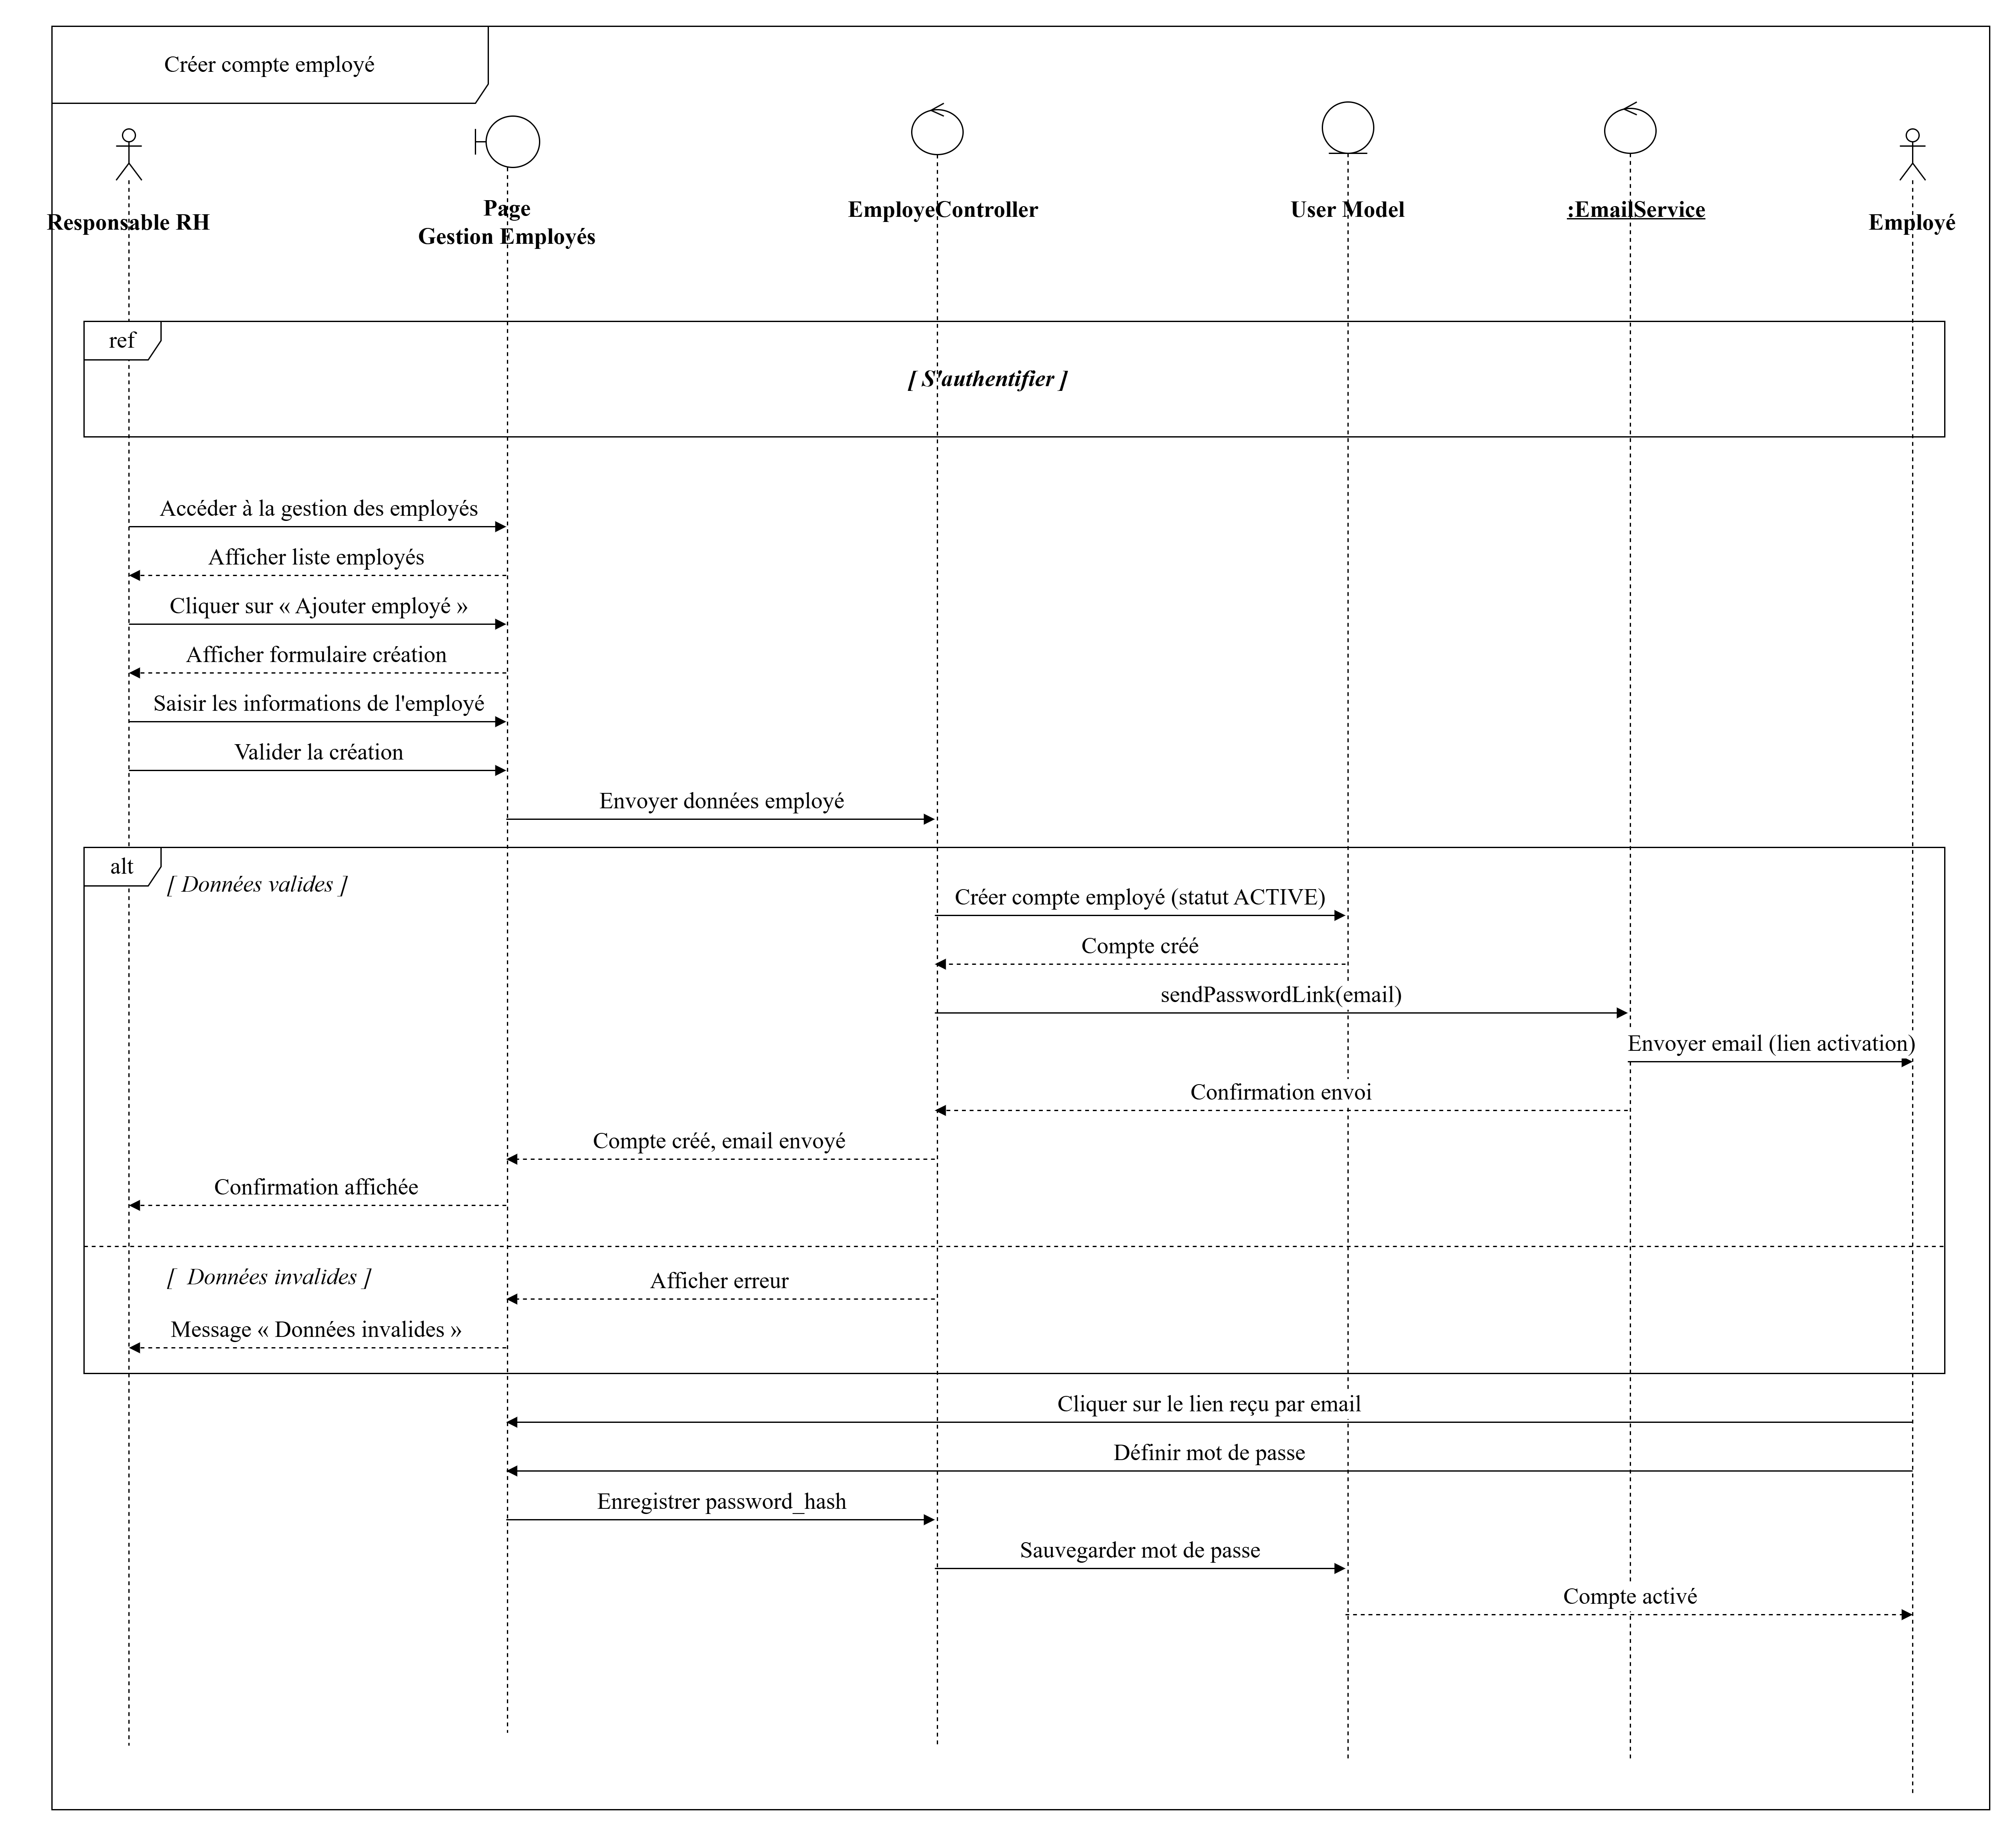
\includegraphics[width=0.9\textwidth]{projet/images/img sequence s1/creer_compte_employe.png}
    \caption{Diagramme de séquence du cas d'utilisation « Créer compte employé »}
\end{figure}


\subsubsection*{Diagramme de séquence du cas d'utilisation « Supprimer compte employé »}

Ce diagramme présente la suppression d'un compte employé par le Responsable RH. Après sélection du compte, le système demande une confirmation avant de procéder à la suppression définitive des données associées.

\begin{figure}[H]
    \centering
    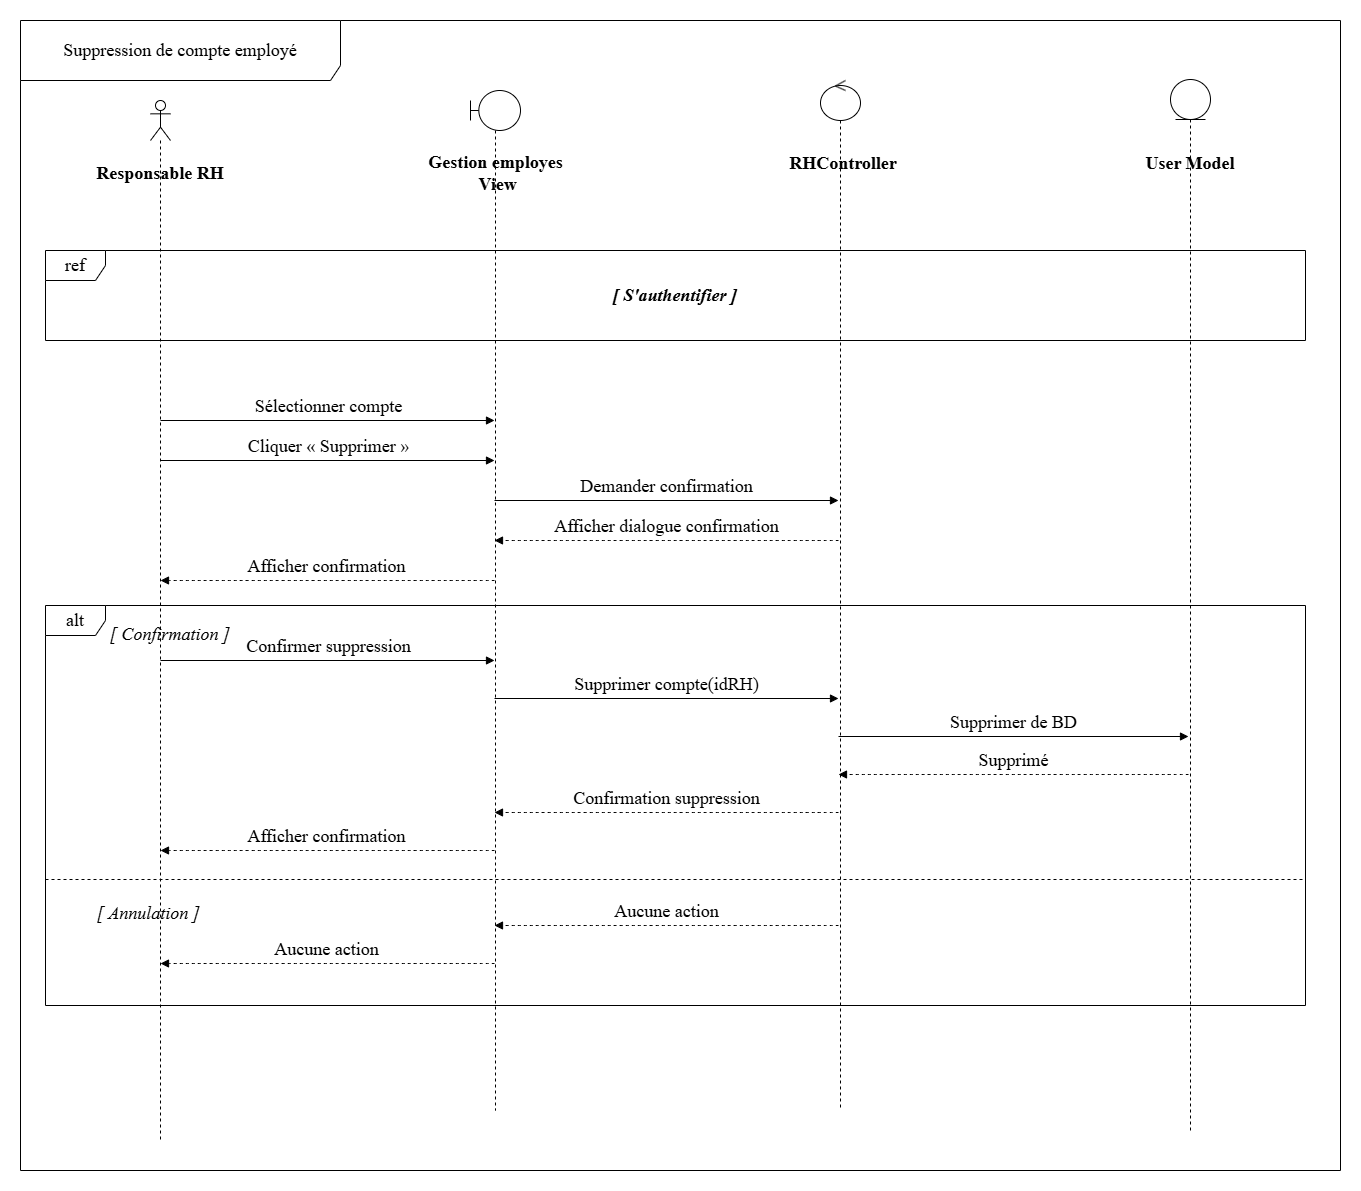
\includegraphics[width=0.9\textwidth]{projet/images/img sequence s1/sup.drawio.png}
    \caption{Diagramme de séquence du cas d'utilisation « Supprimer compte employé »}
\end{figure}


\subsubsection*{Diagramme de séquence du cas d'utilisation « Modifier compte Responsable RH »}

Ce diagramme décrit la modification des informations d'un compte Responsable RH par l'Administrateur. Il sélectionne le compte, met à jour les champs souhaités et le système enregistre les modifications après validation.

\begin{figure}[H]
    \centering
    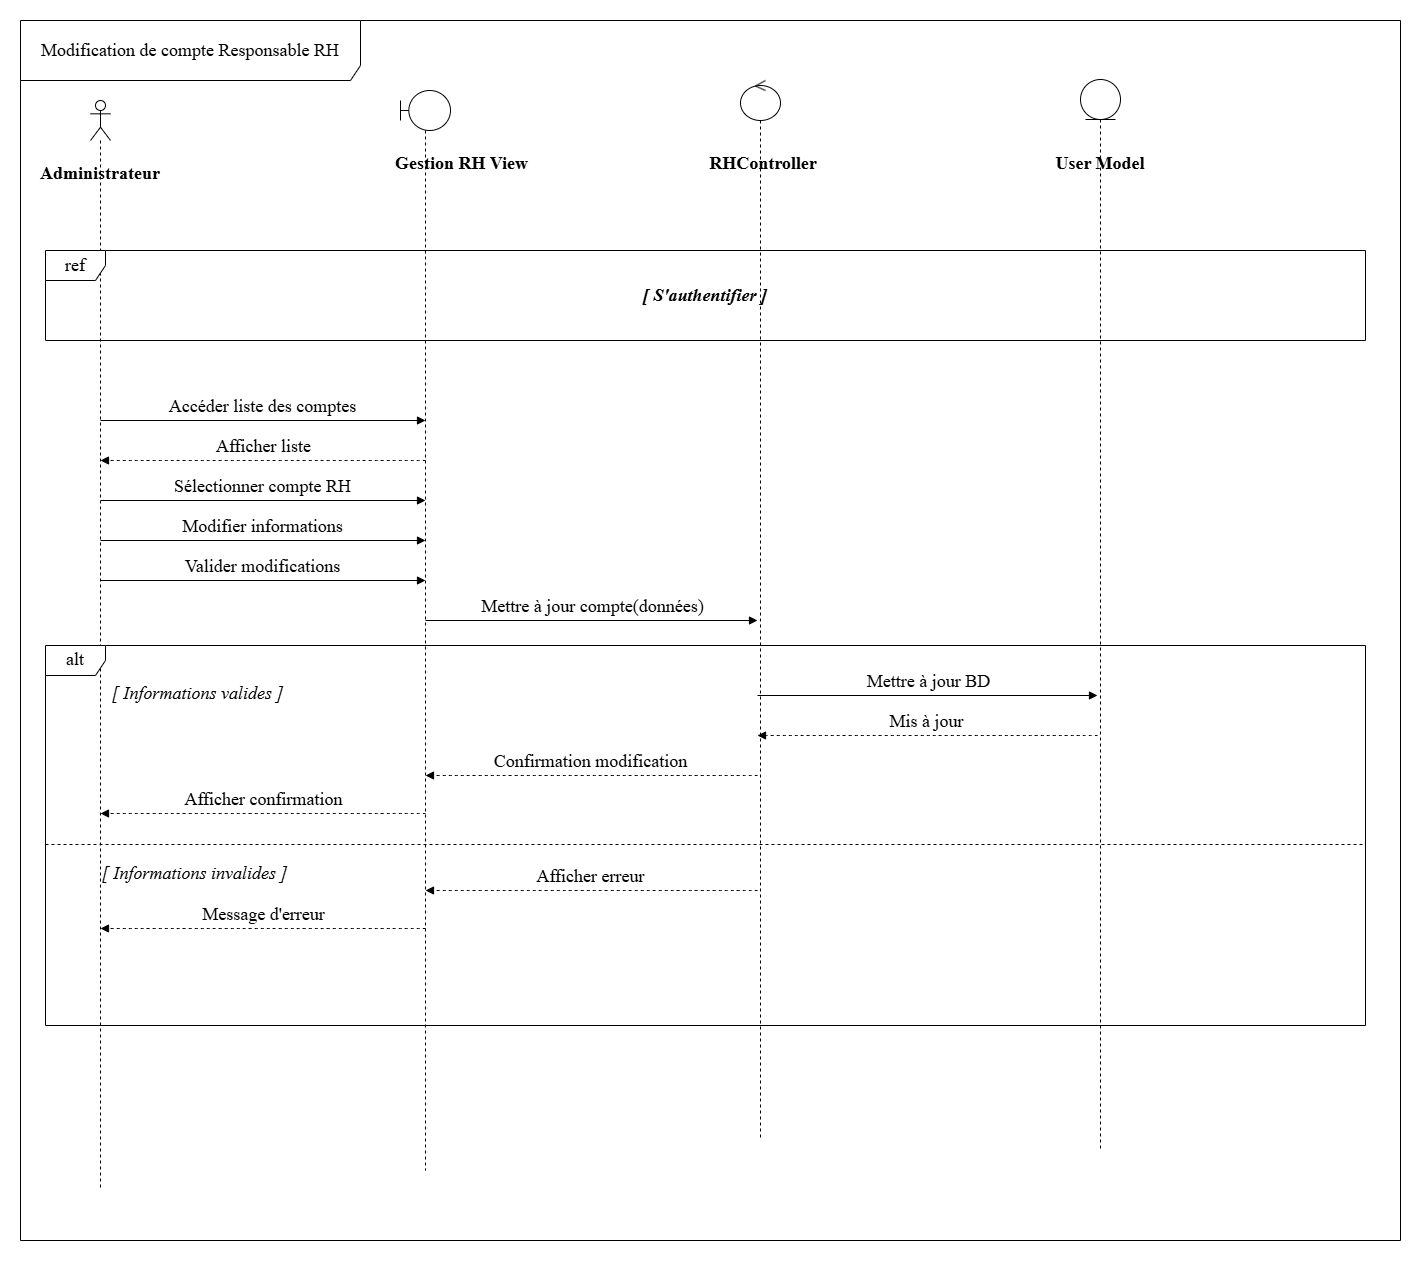
\includegraphics[width=0.9\textwidth]{projet/images/img sequence s1/modifier_compte_rhg.drawio.png}
    \caption{Diagramme de séquence du cas d'utilisation « Modifier compte Responsable RH »}
\end{figure}


\subsubsection{Diagramme de classe du sprint 1}

Ce diagramme de classe illustre la structure du module de gestion des accès et des comptes utilisateurs du système, en affichant les différentes classes, leurs attributs et les relations entre Administrateur, Responsable RH et Employé.

\begin{figure}[H]
    \centering
    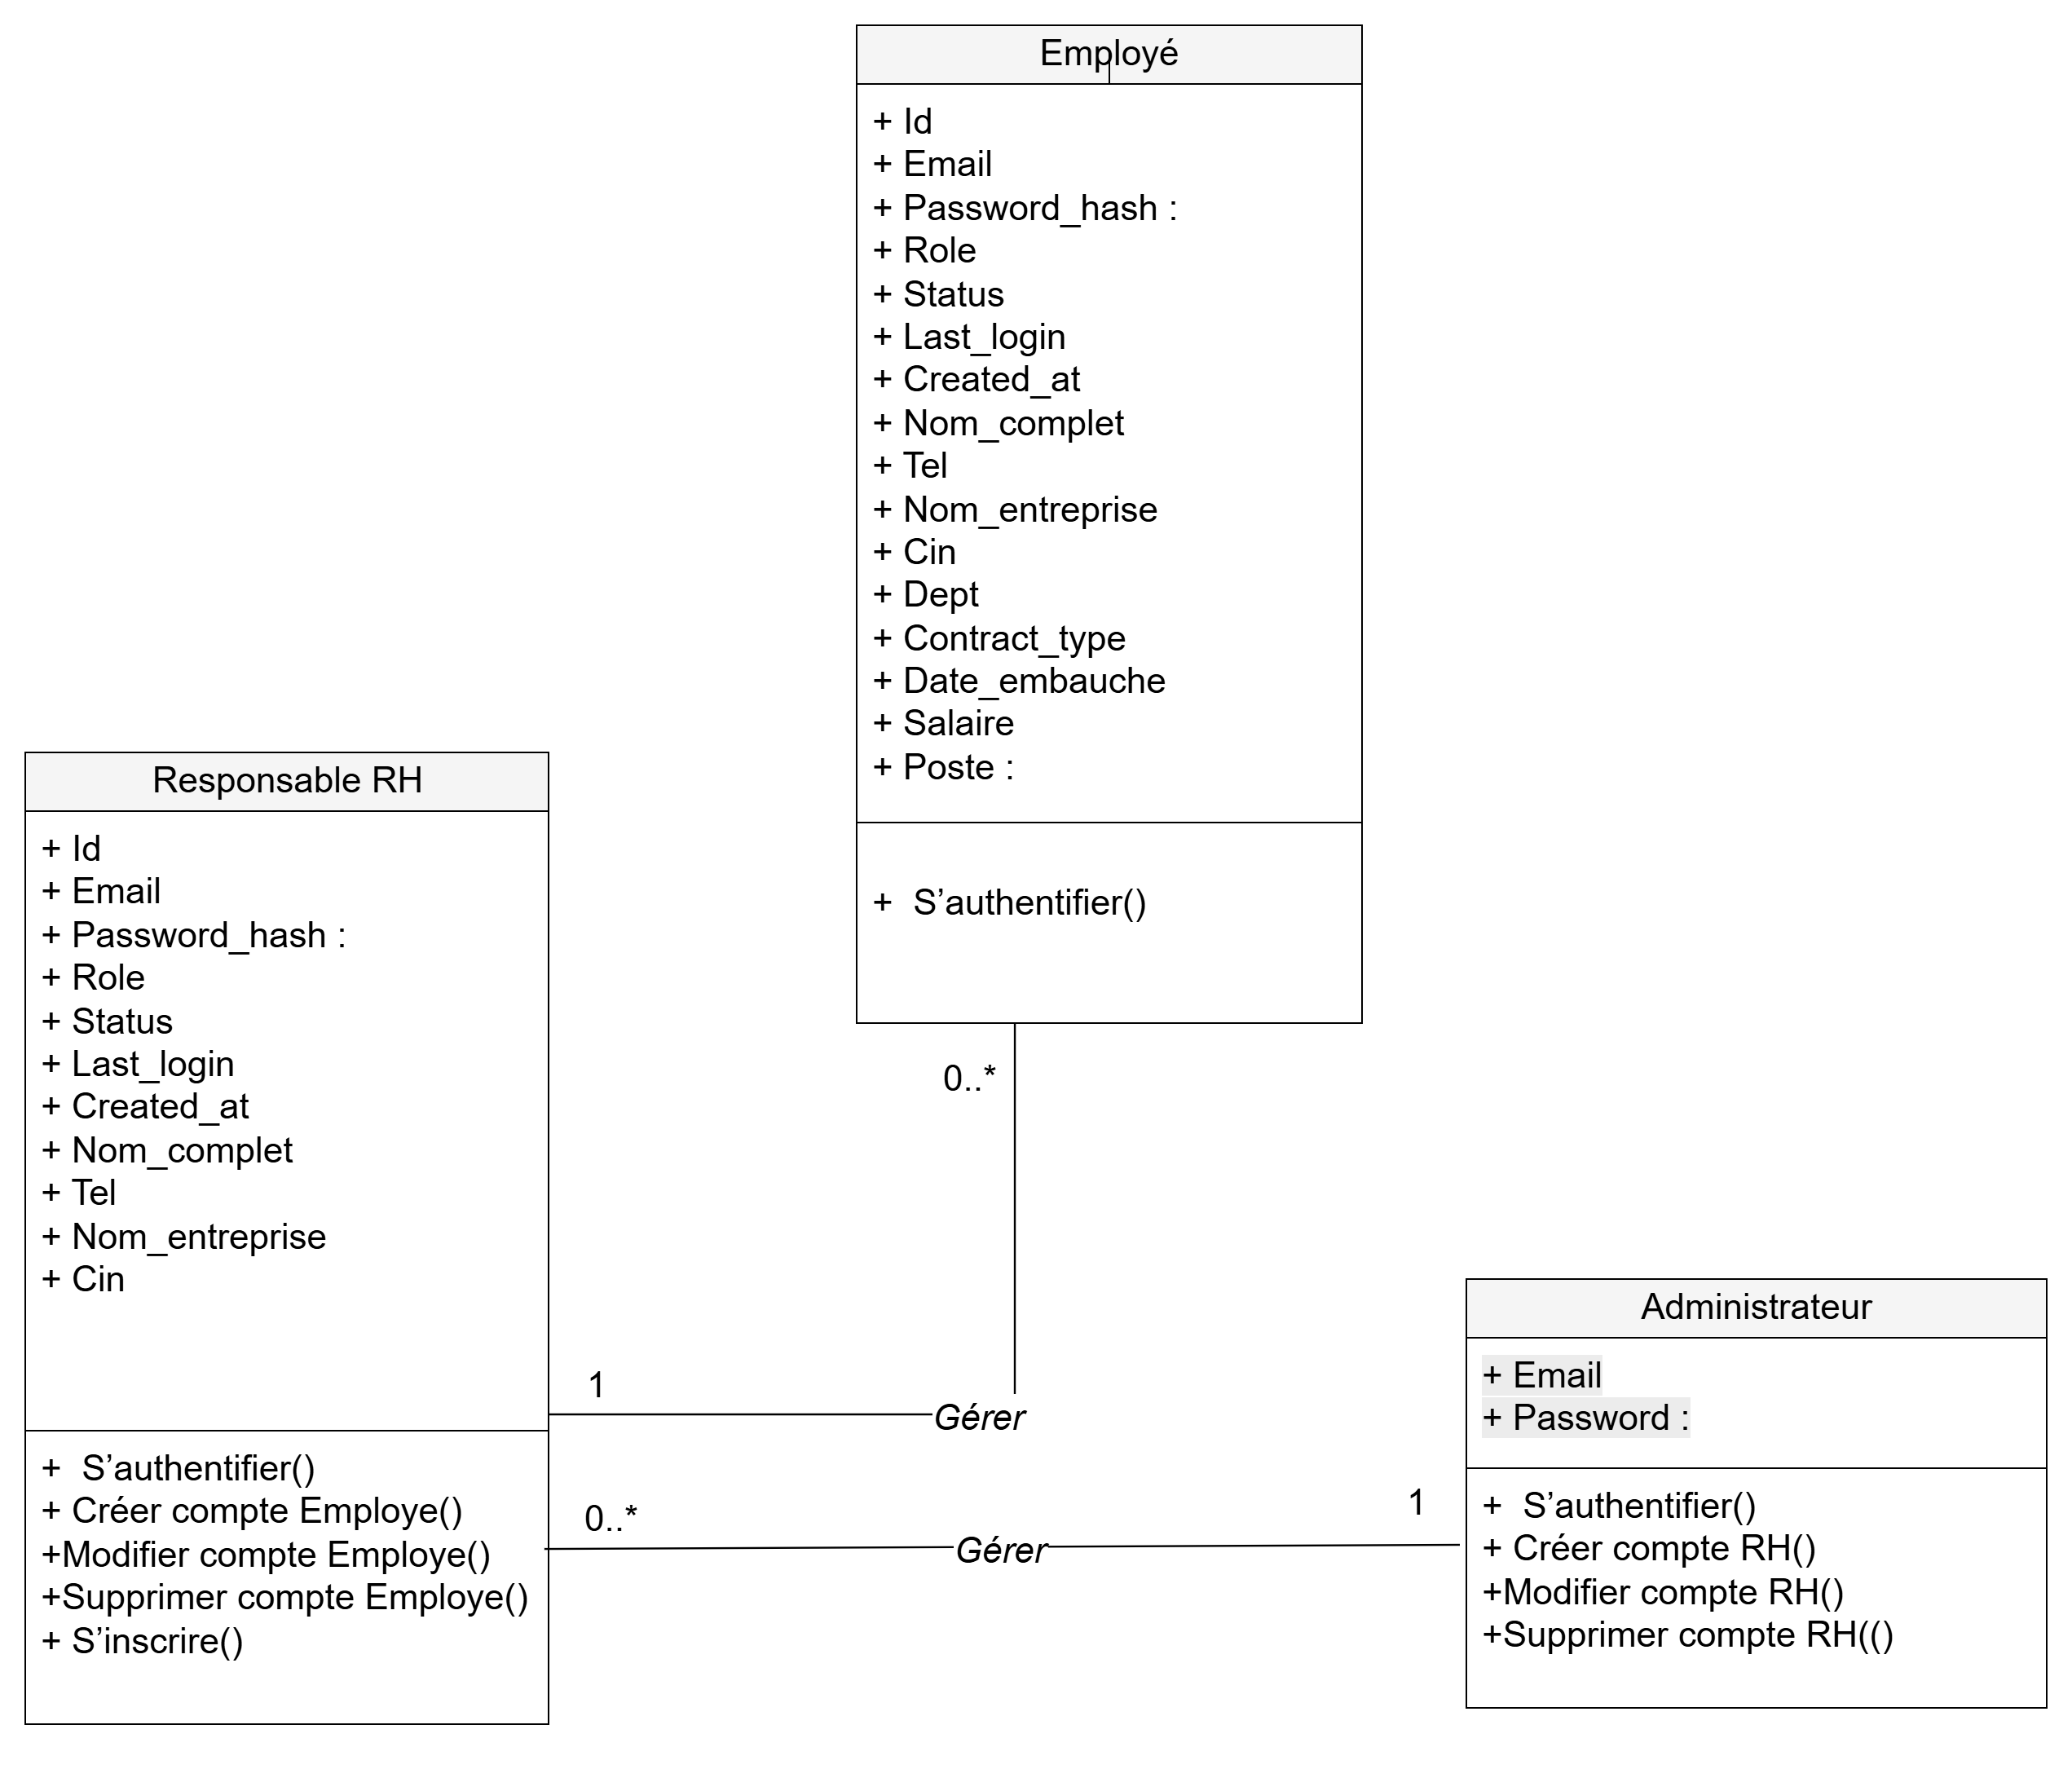
\includegraphics[width=0.9\textwidth]{projet/images/classe finale/diagramme_de_classe_s1.png}
    \caption{Diagramme de classe du sprint 1}
    \label{fig:classe1}
\end{figure}


%============================================================
\subsection{Interfaces réalisées pour le sprint 1}
%============================================================

\subsubsection*{Interface d'authentification}

Cette interface présente la page d'authentification. En effet, chaque utilisateur doit saisir son login et son mot de passe.

\begin{figure}[H]
    \centering
    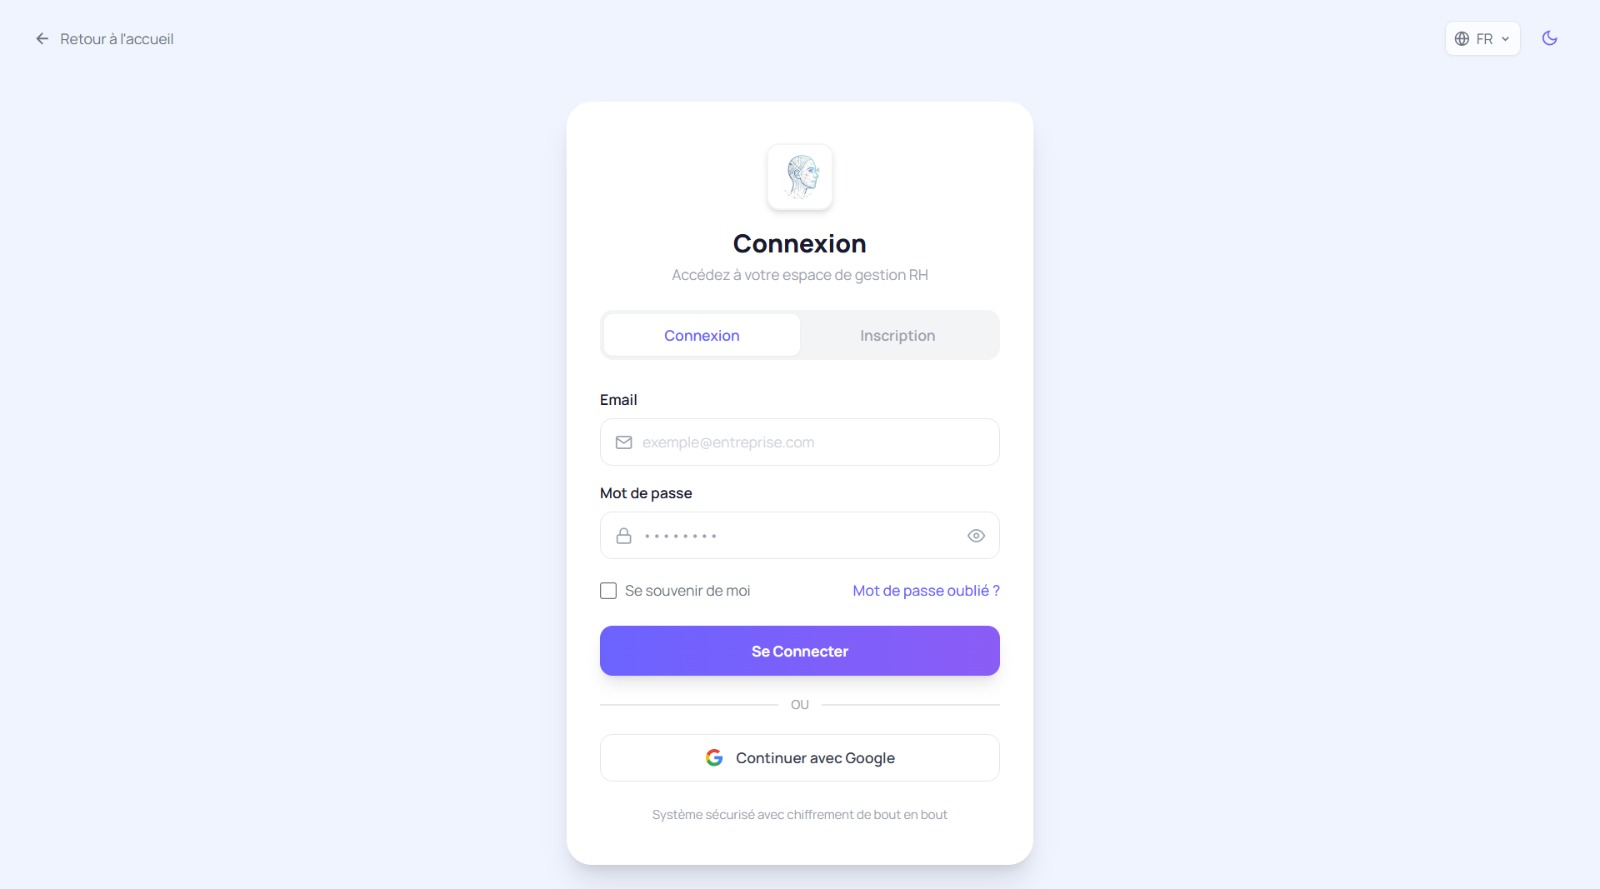
\includegraphics[width=0.9\textwidth]{projet/images/interface/s1/connexion.jpeg}
    \caption{Interface d'authentification}
    \label{fig:interface1}
\end{figure}


\subsubsection*{Interface d'inscription}

Cette interface présente la page d'inscription. En effet, le Responsable RH doit saisir les informations pour créer un nouveau compte.

\begin{figure}[H]
    \centering
    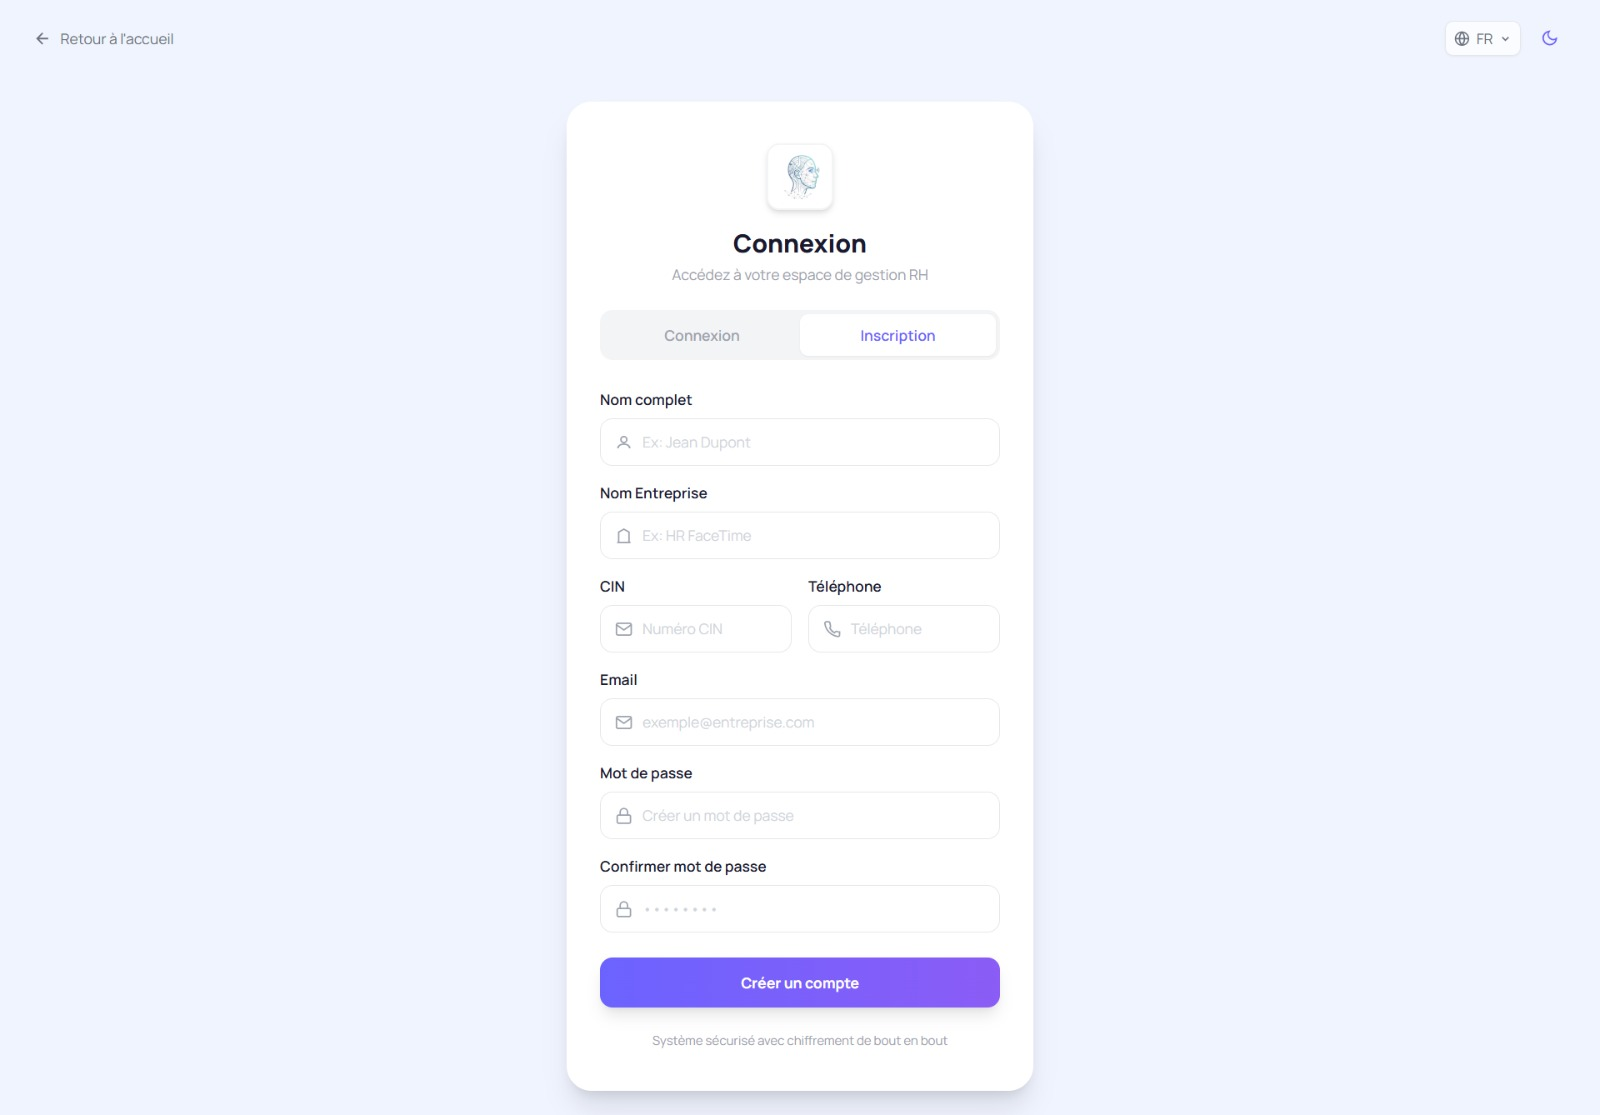
\includegraphics[width=0.9\textwidth]{projet/images/interface/s1/ins.jpeg}
    \caption{Interface d'inscription}
    \label{fig:interface2}
\end{figure}





\subsubsection*{Interface Gérer les comptes employés}

Cette interface permet au Responsable RH de gérer les comptes des employés (création, modification, suppression).

\begin{figure}[H]
    \centering
    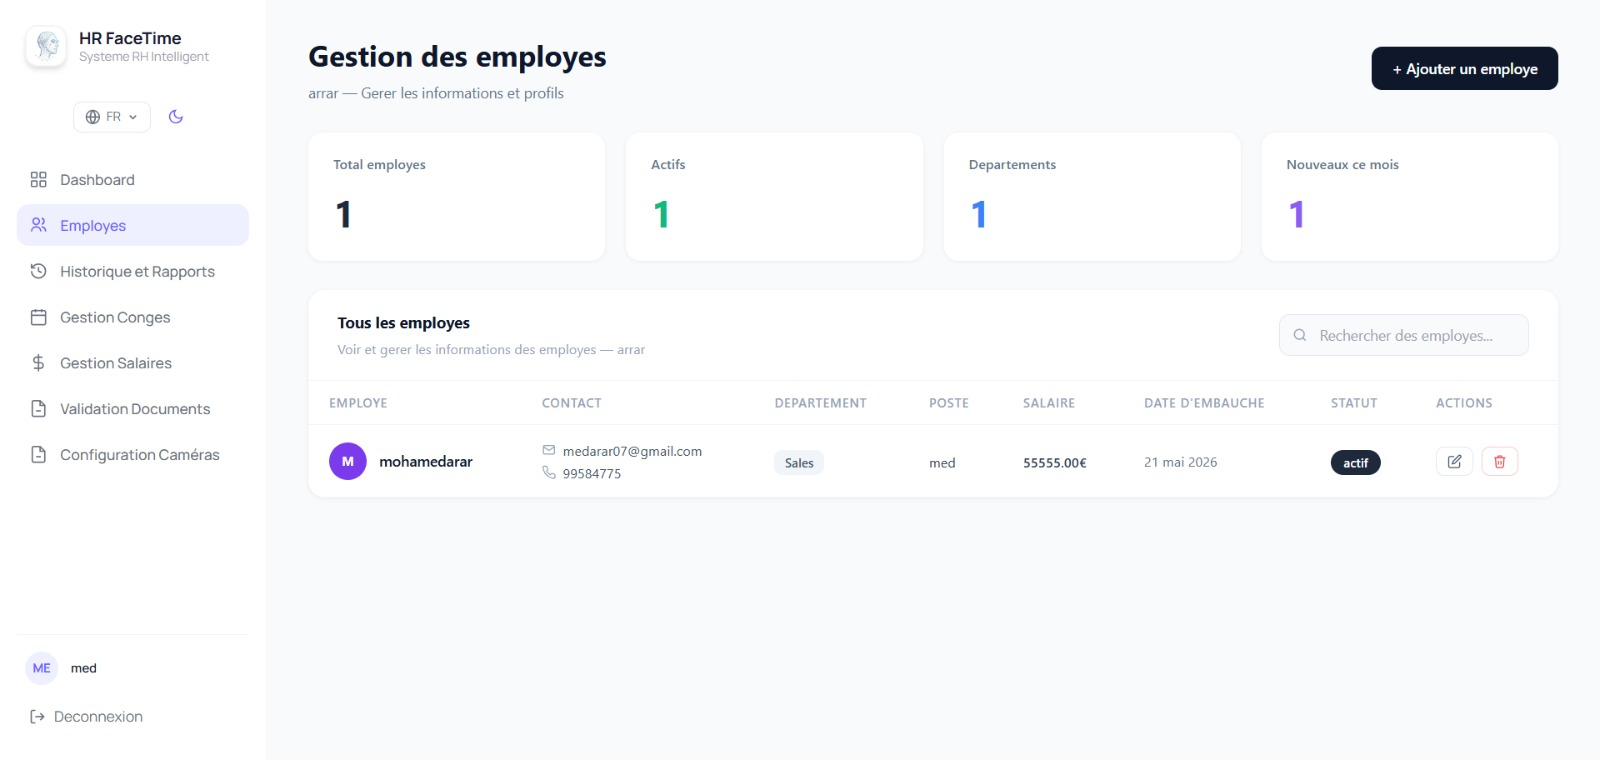
\includegraphics[width=0.9\textwidth]{projet/images/interface/s1/gestion employe.jpeg}
    \caption{Interface Gérer les comptes employés}
    \label{fig:interface4}
\end{figure}


\subsubsection*{Interface Gérer les comptes Responsables RH}

Cette interface permet à l'Administrateur de gérer les comptes des responsables RH (création, modification, suppression).

\begin{figure}[H]
    \centering
    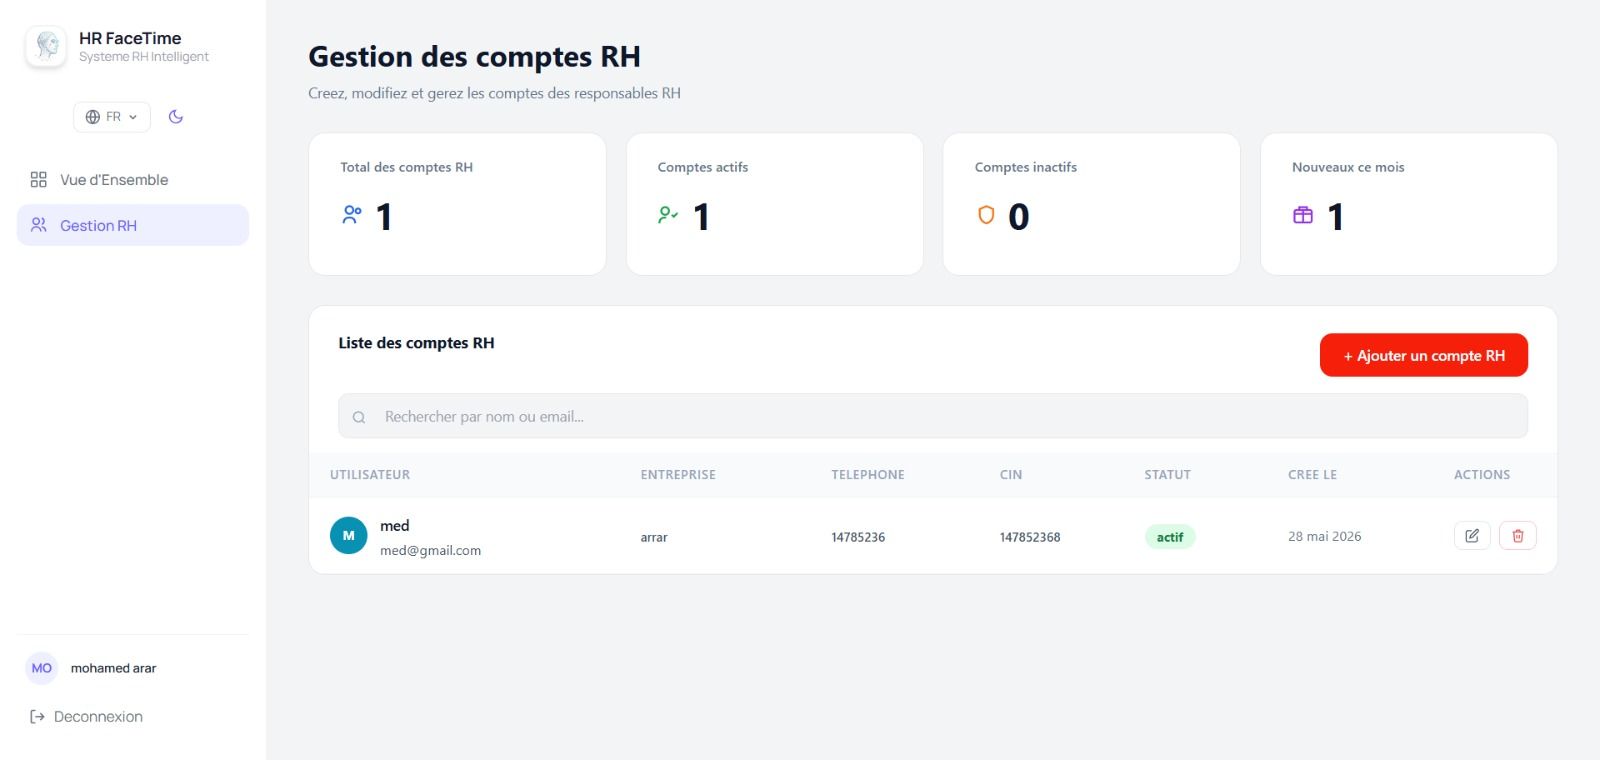
\includegraphics[width=0.9\textwidth]{projet/images/interface/s1/gestion rh.jpeg}
    \caption{Interface Gérer les comptes Responsables RH}
    \label{fig:interface5}
\end{figure}


%============================================================
\section{Sprint 2 : Pointage Intelligent et Suivi de Présence}
%============================================================

Ce sprint consiste à concevoir le module de pointage intelligent utilisant la reconnaissance faciale, afin d'identifier automatiquement les employés et de suivre leur présence dans l'entreprise.

\subsection{Objectif du sprint 2}

L'objectif de ce sprint est d'implémenter le pointage automatique par reconnaissance faciale, de connecter les caméras et de permettre le suivi des présences, absences et informations des employés.

\subsection{Durée du sprint 2}

\begin{itemize}
    \item \textbf{Date de début du sprint} : 12/03/2026
    \item \textbf{Date de fin du sprint} : 06/04/2026
\end{itemize}

\subsection{Backlog du sprint 2}
Ce tableau liste les cinq user stories du sprint 2, portant sur la connexion des caméras, l'enregistrement du visage, la modification des informations personnelles, la consultation des absences et le pointage facial. Les priorités élevées reflètent la complexité technique liée à l'intelligence artificielle et à la reconnaissance faciale.

\begin{longtable}{|>{\centering\arraybackslash}m{0.5cm}|
    >{\centering\arraybackslash}m{3cm}|
    >{\centering\arraybackslash}m{2.5cm}|
    >{\centering\arraybackslash}m{3cm}|
    >{\centering\arraybackslash}m{3cm}|
    >{\centering\arraybackslash}m{0.7cm}|
    >{\centering\arraybackslash}m{0.9cm}|}
\hline
\textbf{ID} & \textbf{User Story} & \textbf{En tant que} & \textbf{Je veux} & \textbf{Afin de} & \textbf{P} & \textbf{C} \\
\hline
\endfirsthead
\hline
\textbf{ID} & \textbf{User Story} & \textbf{En tant que} & \textbf{Je veux} & \textbf{Afin de} & \textbf{P} & \textbf{C} \\
\hline
\endhead
10 & Connecter la plateforme aux caméras & Responsable RH & configurer et connecter les caméras    & activer le pointage automatique     & 5 & 5 \\ \hline
22 & Enregistrer le visage               & Employé        & enregistrer mon visage                 & permettre le pointage automatique   & 5 & 5 \\ \hline
23 & Modifier infos personnelles         & Employé        & modifier mes informations personnelles & maintenir mes données à jour        & 3 & 2 \\ \hline
24 & Consulter ses absences              & Employé        & consulter mes absences                 & suivre ma présence                  & 3 & 2 \\ \hline
30 & Pointage faciale               & Employé        & pointer ma présence par reconnaissance faciale & automatiser le pointage et éviter les oublis de pointage & 5 & 5 \\ \hline
\caption{Backlog Sprint 2 — Pointage Intelligent \& Présence}
\end{longtable}


%============================================================
\subsection{Spécification fonctionnelle détaillée}
%============================================================

\subsubsection*{Diagramme de cas d'utilisation du sprint 2}
Ce diagramme présente les interactions entre le Responsable RH et l'Employé avec les fonctionnalités du sprint 2, notamment la configuration des caméras et les différentes actions liées au pointage intelligent par reconnaissance faciale.

\begin{figure}[H]
    \centering
    
\includegraphics[width=0.9\textwidth]{projet/images/usecase/sprint2/sprint2.drawio.png}
    \caption{Diagramme de Cas d'utilisation du Sprint 2}
    \label{fig:usecase4}
\end{figure}


\subsubsection*{Description textuelle : cas d'utilisation « Connecter la plateforme aux caméras »}
Ce tableau décrit les étapes de configuration et de connexion des caméras par le Responsable RH, depuis l'accès au module jusqu'à l'activation du pointage automatique, ainsi que le scénario d'exception en cas d'échec de connexion.

\begin{longtable}{|p{5cm}|p{11cm}|}
\hline
\textbf{Nom du cas d'utilisation} & \textbf{Connecter la plateforme aux caméras} \\ \hline
\textbf{Acteurs}                  & Responsable RH \\ \hline
\textbf{Objectif}                 & Configurer et connecter les caméras \\ \hline
\textbf{Préconditions}            & Le Responsable RH doit être authentifié \\ \hline
\textbf{Scénario nominal} &
1. Le Responsable RH accède aux « Configuration Caméras ». \newline
2. Il choisit l'option « Détecter les caméras ». \newline
3. Il définit la caméra d'entrée et la caméra de sortie. \newline
4. Il valide la configuration. \newline
5. Le système connecte les caméras et active le pointage automatique. \\ \hline
\textbf{Scénario d'exception} &
5.1 Si la connexion échoue, le système demande de réessayer. \\ \hline
\textbf{Post-condition} & Les caméras sont connectées et le pointage automatique est activé. \\ \hline
\caption{Description textuelle du cas d'utilisation « Connecter la plateforme aux caméras »}
\end{longtable}


\subsubsection*{Description textuelle : cas d'utilisation « Enregistrer le visage »}
Ce tableau présente le processus d'enregistrement biométrique du visage d'un employé lors de sa première connexion, incluant la capture par caméra et le stockage des données faciales dans le système pour permettre le pointage automatique.

\begin{longtable}{|p{5cm}|p{11cm}|}
\hline
\textbf{Nom du cas d'utilisation} & \textbf{Enregistrer le visage} \\ \hline
\textbf{Acteurs}                  & Employé \\ \hline
\textbf{Objectif}                 & Enregistrer le visage pour le pointage automatique \\ \hline
\textbf{Préconditions}            & L'employé doit être authentifié \\ \hline
\textbf{Scénario nominal} &
1. L'employé saisit ses informations de connexion. \newline
2. Le système vérifie les informations. \newline
3. Lors de la première connexion, le système demande l'enregistrement du visage. \newline
4. L'employé autorise l'accès à la caméra. \newline
5. La caméra capture le visage. \newline
6. Le système enregistre les données. \newline
7. L'employé accède à son espace personnel. \\ \hline
\textbf{Scénario d'exception} &
3.1 Si la capture échoue, le système demande de recommencer. \\ \hline
\textbf{Post-condition} & Le visage est enregistré pour le pointage automatique. \\ \hline
\caption{Description textuelle du cas d'utilisation « Enregistrer le visage »}
\end{longtable}


\subsubsection*{Description textuelle : cas d'utilisation « Modifier infos personnelles »}
Ce tableau décrit les étapes permettant à l'employé de consulter et de mettre à jour ses informations personnelles depuis son profil, ainsi que le scénario d'exception déclenché en cas de saisie de données invalides.

\begin{longtable}{|p{5cm}|p{11cm}|}
\hline
\textbf{Nom du cas d'utilisation} & \textbf{Modifier infos personnelles} \\ \hline
\textbf{Acteurs}                  & Employé \\ \hline
\textbf{Objectif}                 & Modifier ses informations personnelles \\ \hline
\textbf{Préconditions}            & Employé authentifié \\ \hline
\textbf{Scénario nominal} &
1. L'employé accède à « Mon Profil ». \newline
2. Il visualise ses données personnelles (nom, email, poste, etc.). \newline
3. Il met à jour les champs souhaités. \newline
4. Il valide les modifications. \newline
5. Le système enregistre les changements. \\ \hline
\textbf{Scénario d'exception} &
3.1 Si les champs sont invalides, le système affiche « Modification impossible ». \\ \hline
\textbf{Post-condition} & Les informations personnelles sont consultées et/ou mises à jour. \\ \hline
\caption{Description textuelle du cas d'utilisation « Modifier infos personnelles »}
\end{longtable}


\subsubsection*{Description textuelle : cas d'utilisation « Consulter mes absences »}
Ce tableau présente le scénario de consultation par l'employé de son historique d'absences et de retards depuis son tableau de bord, avec le cas d'exception affiché en l'absence de données disponibles dans le système.

\begin{longtable}{|p{5cm}|p{11cm}|}
\hline
\textbf{Nom du cas d'utilisation} & \textbf{Consulter mes absences} \\ \hline
\textbf{Acteurs}                  & Employé \\ \hline
\textbf{Objectif}                 & Consulter ses absences et retards \\ \hline
\textbf{Préconditions}            & L'employé doit être authentifié \\ \hline
\textbf{Scénario nominal} &
1. L'employé accède à son tableau de bord. \newline
2. Il consulte la section « Mes Absences ». \newline
3. Le système affiche ses absences . \\ \hline
\textbf{Scénario d'exception} &
2.1 Si aucune donnée n'est disponible, le système affiche un message. \\ \hline
\textbf{Post-condition} & L'employé visualise ses informations de présence. \\ \hline
\caption{Description textuelle du cas d'utilisation « Consulter mes absences et retards »}
\end{longtable}


\subsubsection*{Description textuelle : cas d'utilisation « Pointage Facial »}
Ce tableau détaille le scénario nominal du pointage facial en mode télétravail, couvrant les opérations de check-in et check-out via reconnaissance faciale, ainsi que l'exception déclenchée en cas d'échec d'identification du visage par le système.

\begin{center}
\begin{longtable}{|p{5cm}|p{11cm}|}
\hline
\textbf{Nom du cas d'utilisation} & \textbf{Pointage Facial} \\ \hline

\textbf{Acteurs} & Employé \\ \hline

\textbf{Objectif} & Enregistrer sa présence à distance via la reconnaissance faciale. \\ \hline

\textbf{Préconditions} & L'employé doit être authentifié et son mode de travail doit être défini sur « Télétravail ». \\ \hline

\textbf{Scénario nominal} &

1. L'employé accède à l'interface de pointage. \newline
2. Il clique sur le bouton « Check In ». \newline
3. La caméra s'active et capture son visage. \newline
4. Le système effectue la reconnaissance faciale. \newline
5. Le système enregistre l'heure d'entrée et confirme le pointage. \newline
6. À la fin de sa journée de travail, l'employé clique sur le bouton « Check Out ». \newline
7. La caméra capture à nouveau son visage. \newline
8. Le système vérifie son identité et enregistre l'heure de sortie.
   \\ \hline

\textbf{Scénario d'exception} &
4.1 Si le visage n'est pas reconnu, le système affiche un message d'erreur et refuse le pointage.
\\ \hline

\textbf{Post-condition} & Les heures d'entrée et de sortie de l'employé sont enregistrées.
\\ \hline

\caption{Description textuelle du cas d'utilisation « Pointage Facial en Télétravail »}
\end{longtable}
\end{center}


%============================================================
\subsection{Conception}
%============================================================

Cette section présente les différents diagrammes UML réalisés afin de modéliser le fonctionnement du système, notamment les diagrammes de séquence et les diagrammes de classes, permettant de décrire les interactions entre les acteurs ainsi que la structure globale de l'application.

\subsubsection{Diagrammes de séquence du sprint 2}

\subsubsection*{Diagramme de séquence du cas d'utilisation « Connecter la plateforme aux caméras »}

Ce diagramme illustre la configuration et la connexion des caméras à la plateforme par le Responsable RH. Il saisit les paramètres de connexion, le système établit la liaison avec les caméras et active le module de pointage automatique par reconnaissance faciale.

\begin{figure}[H]
    \centering
    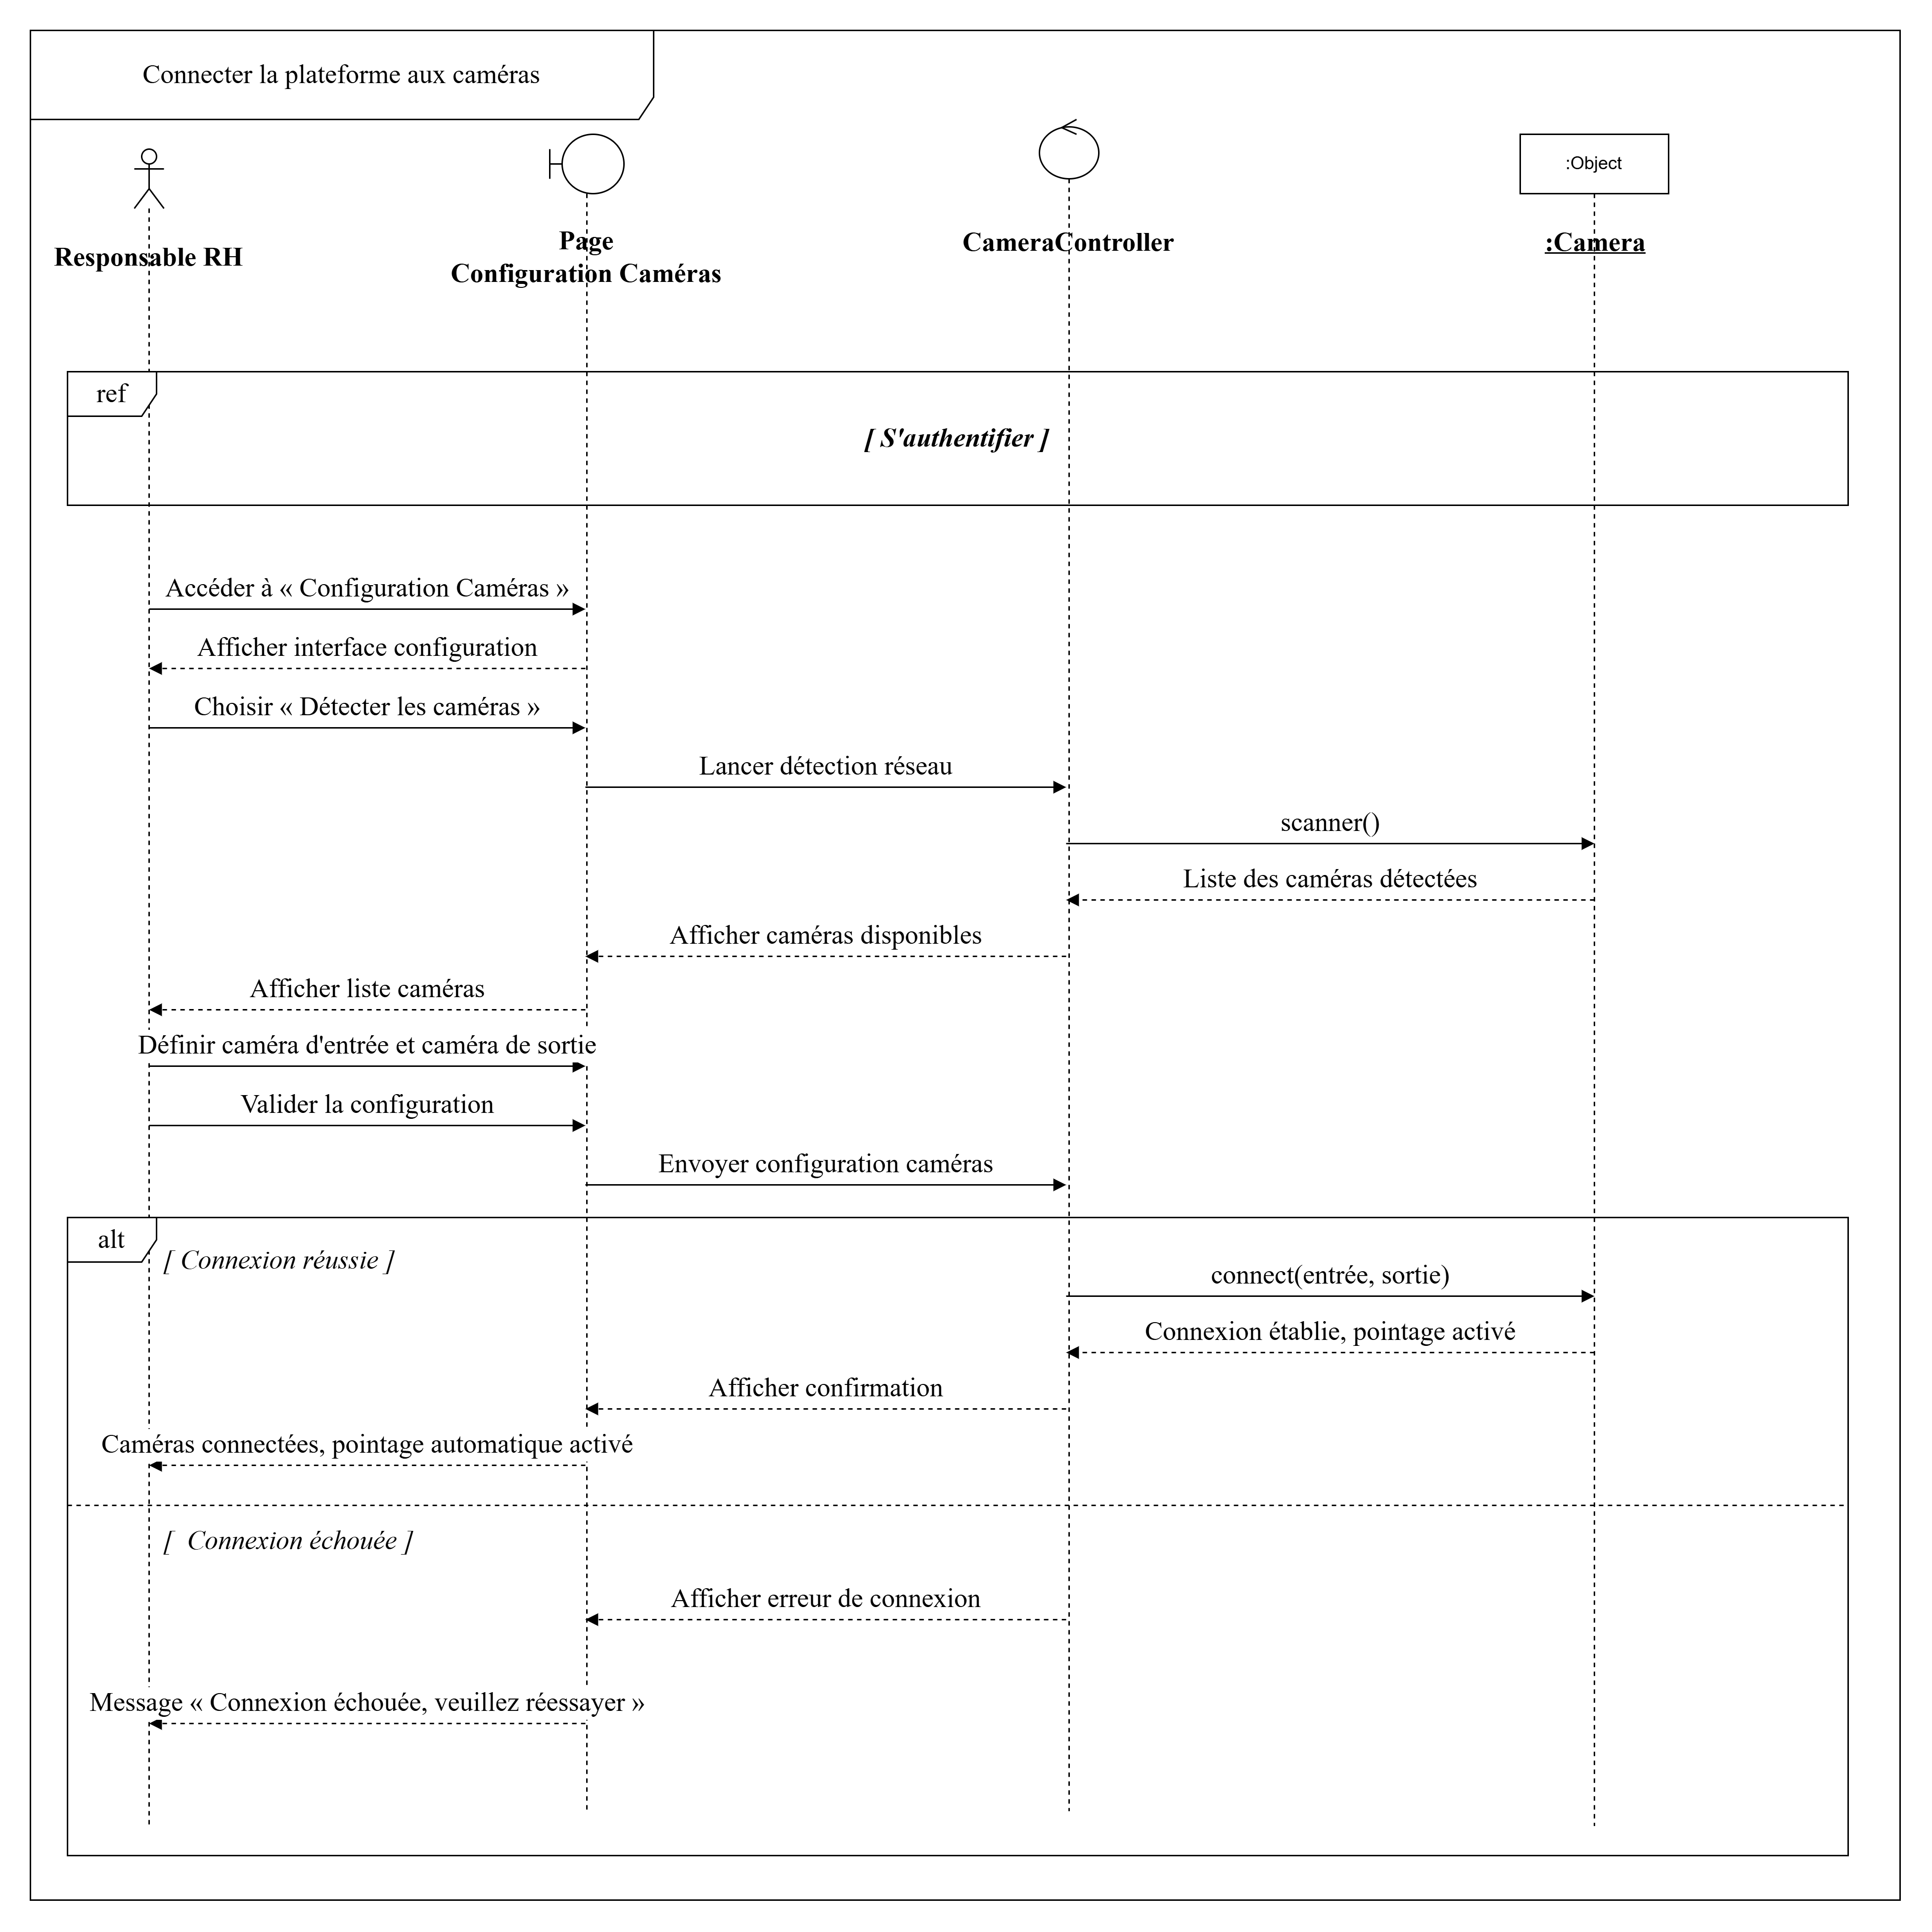
\includegraphics[width=0.85\textwidth]{projet/images/img diag sprint 2/connecter_cameras.png}
    \caption{Diagramme de séquence du cas d'utilisation « Connecter la plateforme aux caméras »}
\end{figure}


\subsubsection*{Diagramme de séquence du cas d'utilisation « Enregistrer le visage »}

Ce diagramme décrit le processus d'enregistrement du visage d'un employé pour le pointage automatique. La caméra capture le visage, le module d'intelligence artificielle traite et enregistre les données biométriques dans la base de données.

\begin{figure}[H]
    \centering
    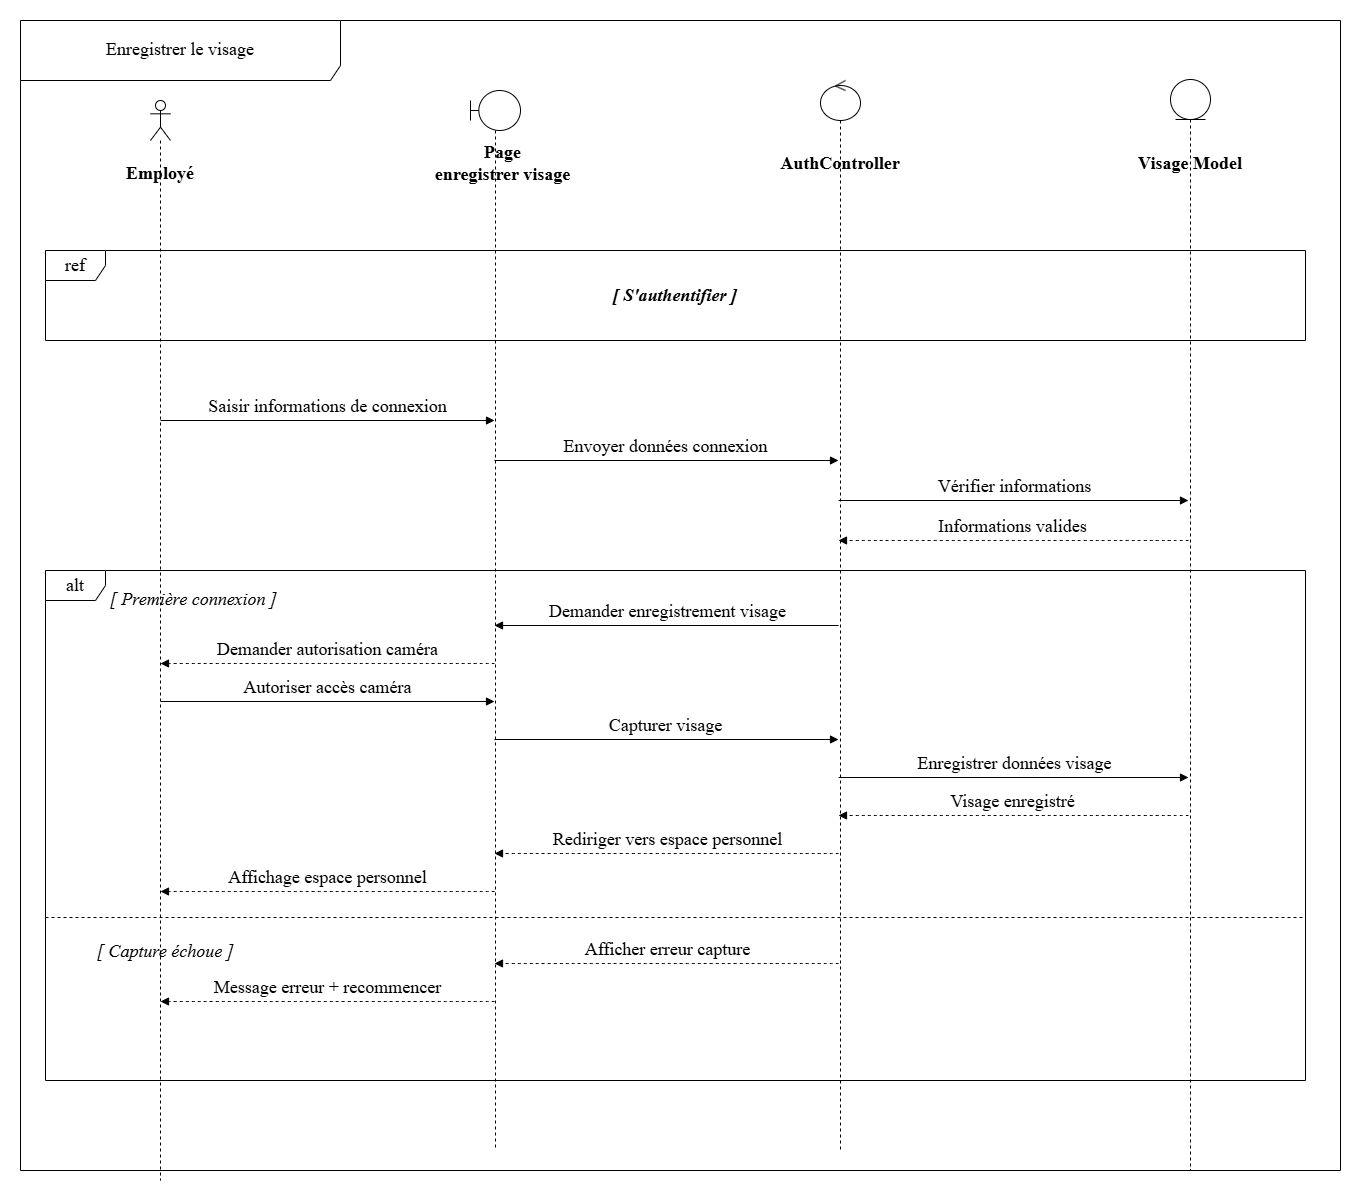
\includegraphics[width=0.85\textwidth]{projet/images/img diag sprint 2/enregister_visage.png}
    \caption{Diagramme de séquence du cas d'utilisation « Enregistrer le visage »}
\end{figure}


\subsubsection*{Diagramme de séquence du cas d'utilisation « Modifier infos personnelles »}

Ce diagramme illustre la mise à jour des informations personnelles par l'employé. Il modifie les champs souhaités, le système vérifie la validité des données saisies et enregistre les modifications avec une confirmation à l'utilisateur.

\begin{figure}[H]
    \centering
    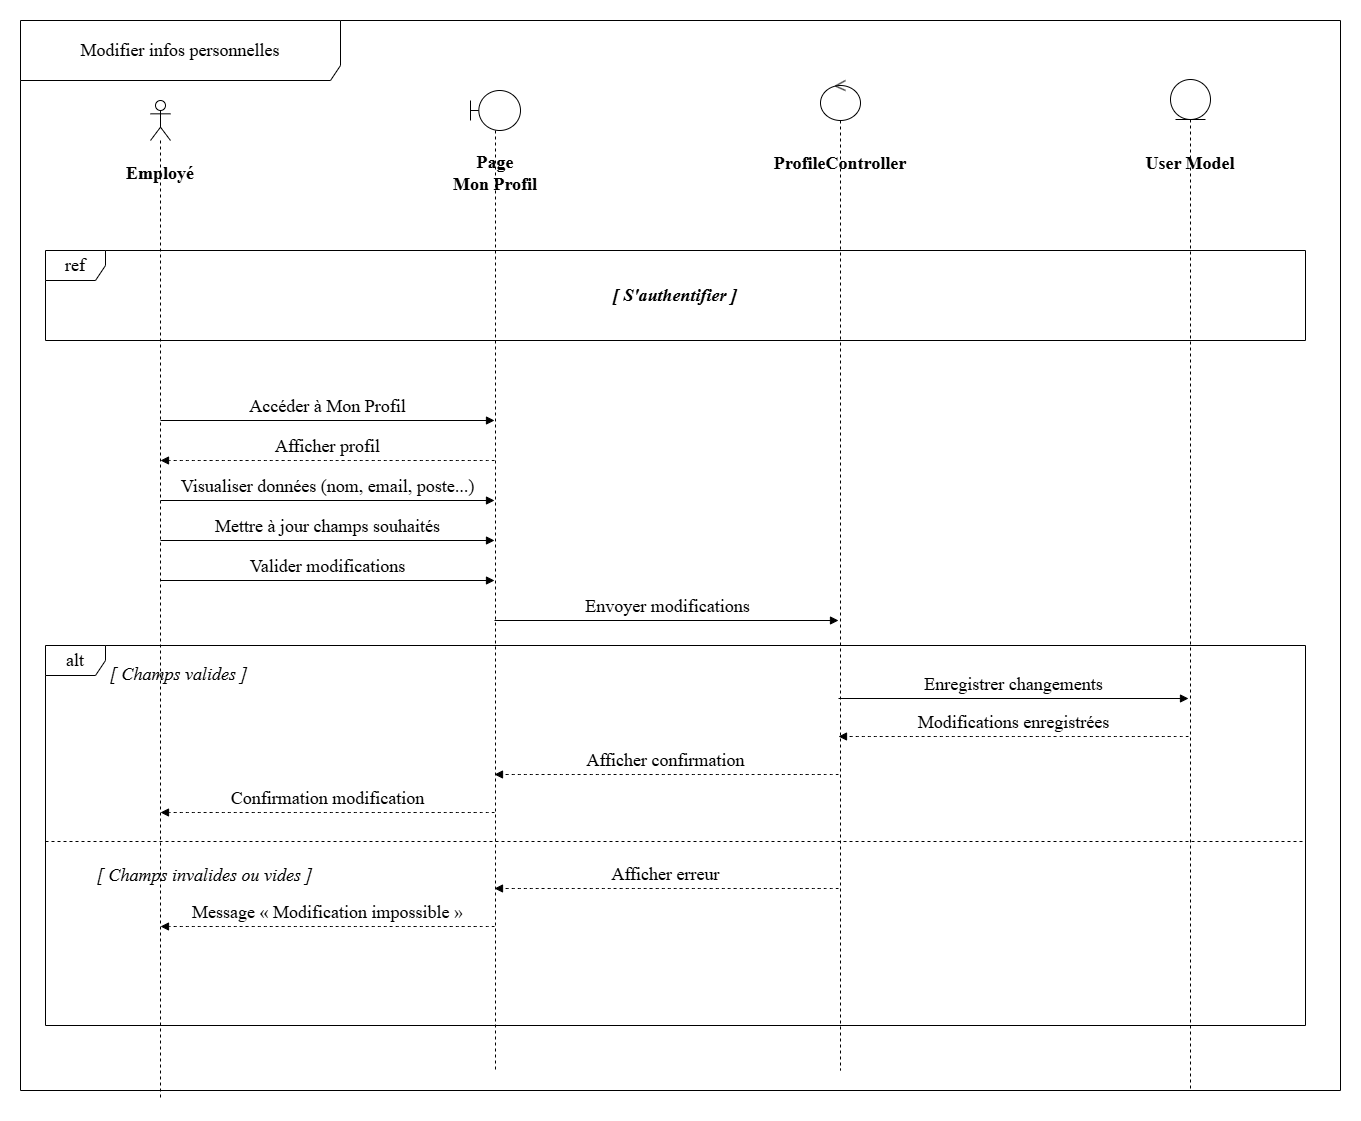
\includegraphics[width=0.85\textwidth]{projet/images/img diag sprint 2/modifier_infos.png}
    \caption{Diagramme de séquence du cas d'utilisation « Modifier infos personnelles »}
\end{figure}

\subsubsection*{Diagramme de séquence du cas d'utilisation « Consulter ses absences »}

Ce diagramme décrit la consultation par l'employé de son historique d'absences et de retards. Il accède à la section dédiée de son tableau de bord, le système interroge la base de données et affiche la liste détaillée des occurrences enregistrées.

\begin{figure}[H]
    \centering
    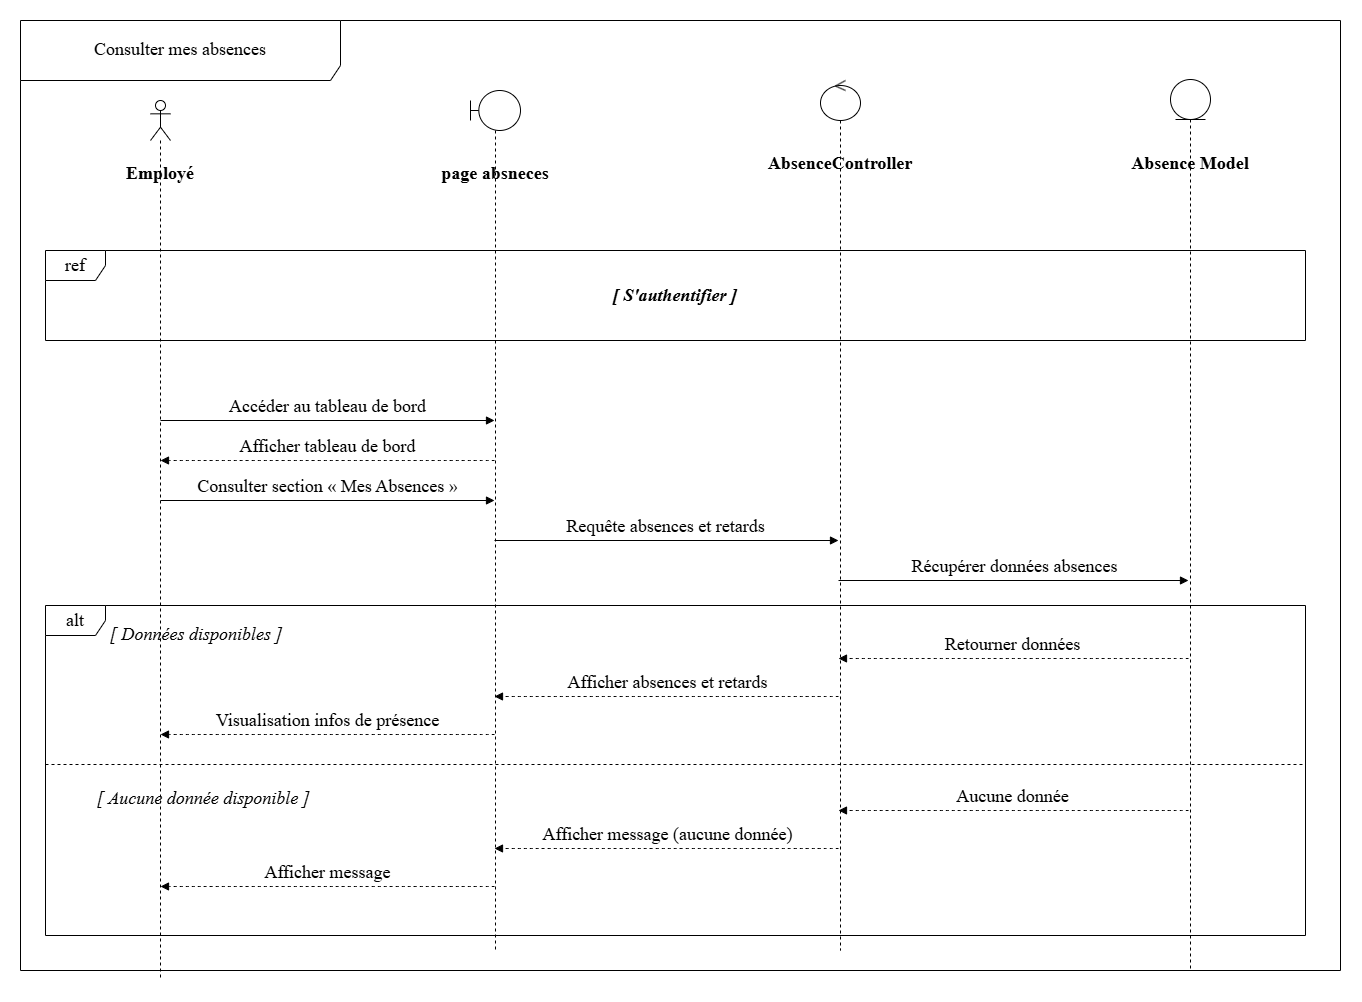
\includegraphics[width=0.85\textwidth]{projet/images/img diag sprint 2/consulter_retard.png}
    \caption{Diagramme de séquence du cas d'utilisation « Consulter ses absences et retards »}
\end{figure}


\subsubsection*{Diagramme de séquence du cas d'utilisation « Pointage facial »}

Le diagramme de pointage facial illustre le processus d'enregistrement de la présence des employés via la reconnaissance faciale, depuis la capture du visage par la caméra jusqu'à la vérification de l'identité et l'enregistrement des heures d'entrée et de sortie dans le système.

\begin{figure}[H]
    \centering
    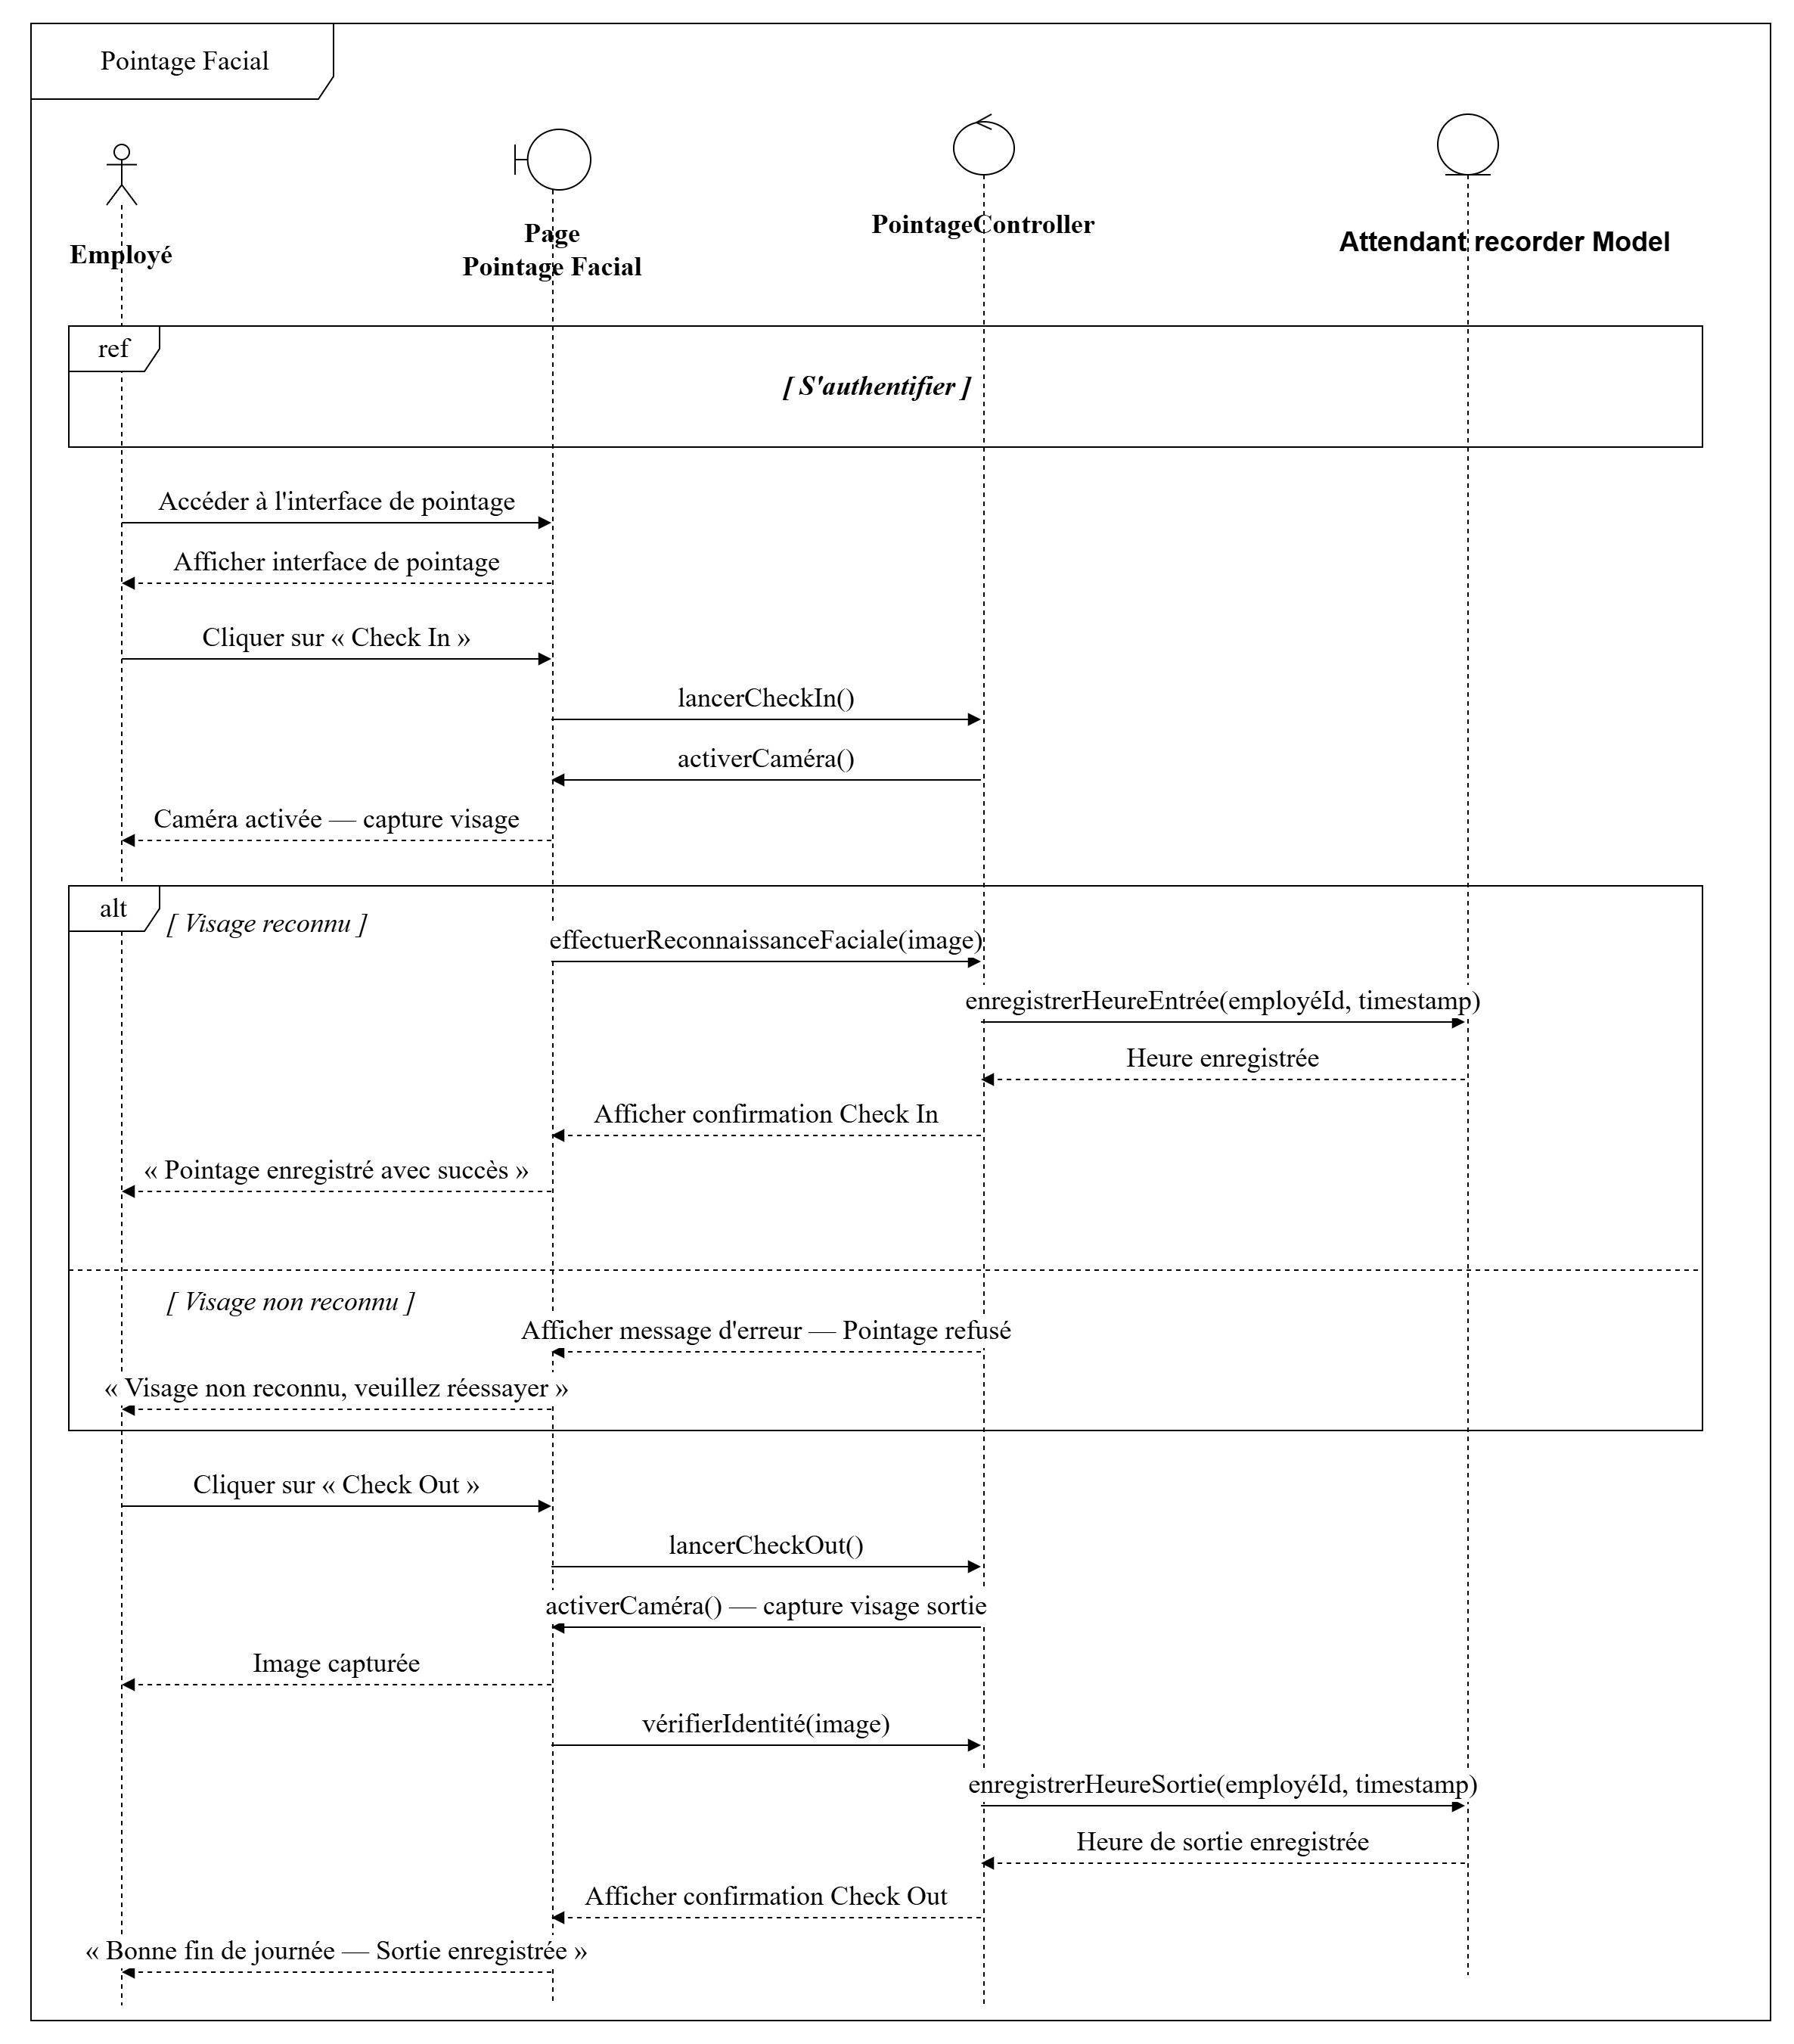
\includegraphics[width=0.85\textwidth]{projet/images/img diag sprint 2/pointage_facial.png}
    \caption{Diagramme de séquence du cas d'utilisation « Pointage facial »}
\end{figure}


\subsubsection{Diagramme de classe du sprint 2}

Ce diagramme de classe illustre la structure des composants liés au pointage intelligent, en montrant les classes Camera, Présence, Absence et leurs attributs respectifs, ainsi que leurs relations avec la classe Employé au sein du système.

\begin{figure}[H]
    \centering
    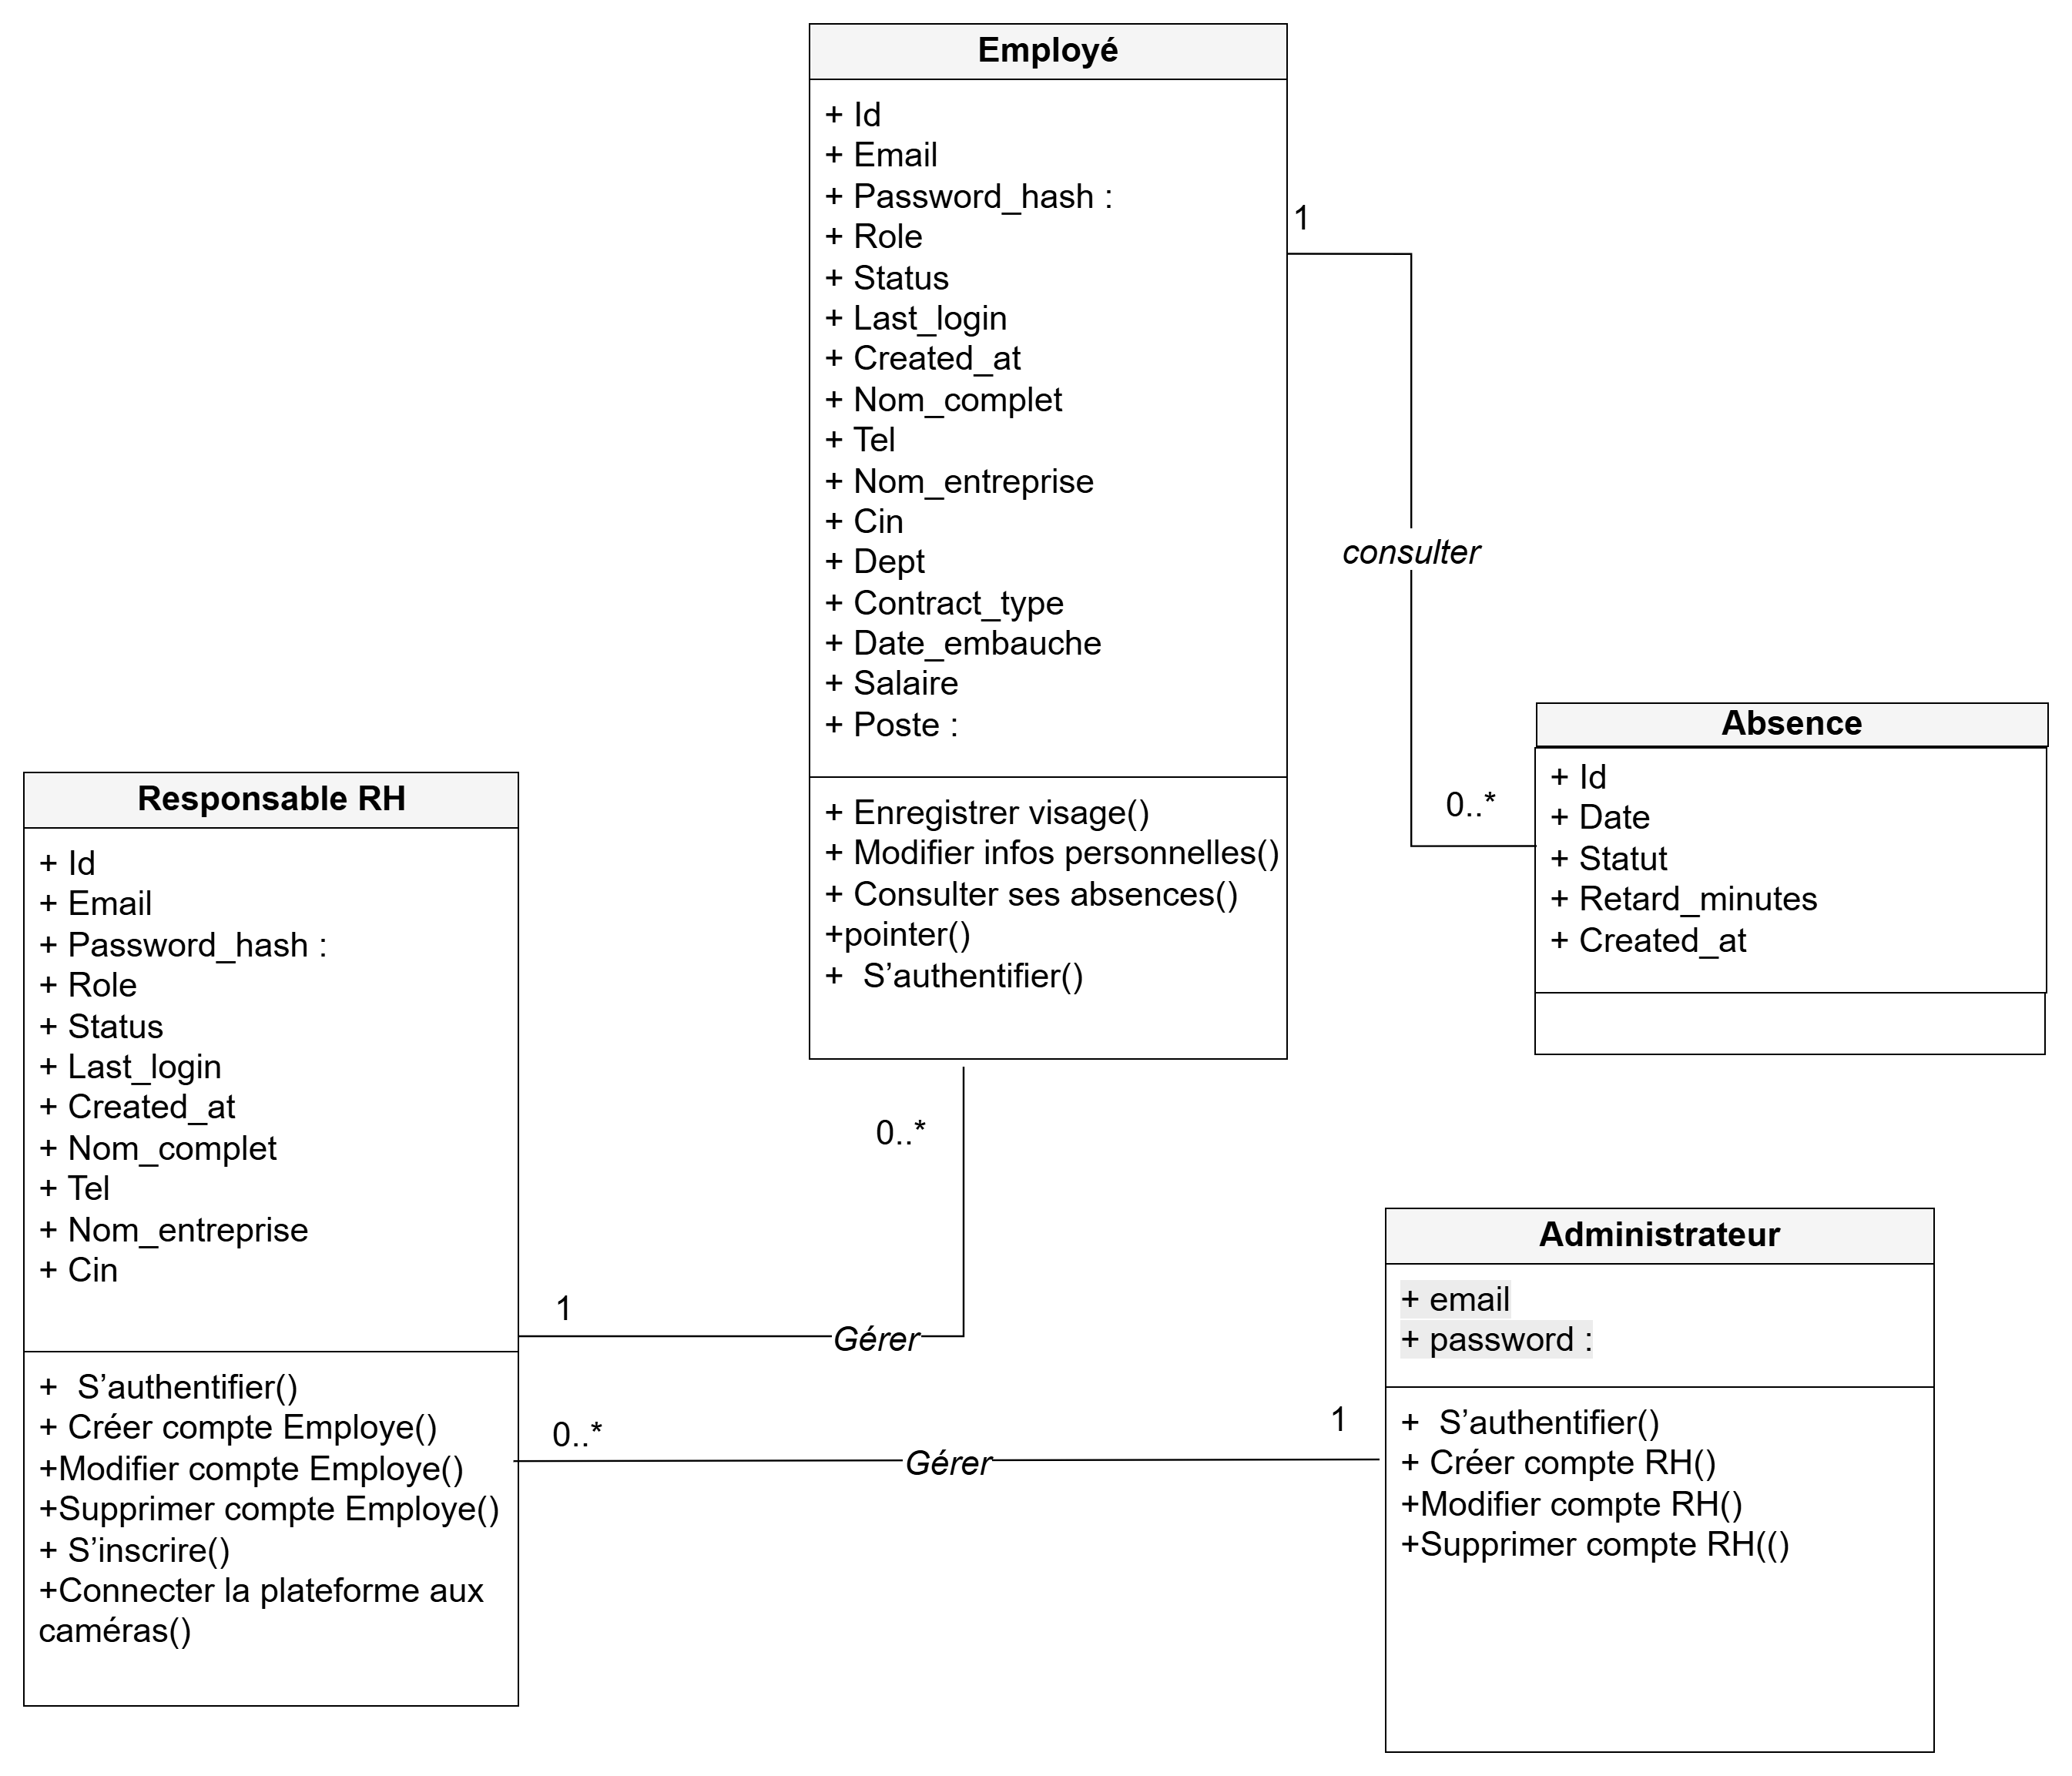
\includegraphics[width=0.85\textwidth]{projet/images/classe finale/daigramme_de_classe_s2.png}
    \caption{Diagramme de classe du sprint 2}
    \label{fig:classe2}
\end{figure}


%============================================================
\subsection{Interfaces réalisées pour le sprint 2}
%============================================================

\subsubsection*{Connecter la plateforme aux caméras}

Cette interface permet de connecter le système aux caméras afin d'activer la capture et la reconnaissance des flux vidéo.

\begin{figure}[H]
    \centering
    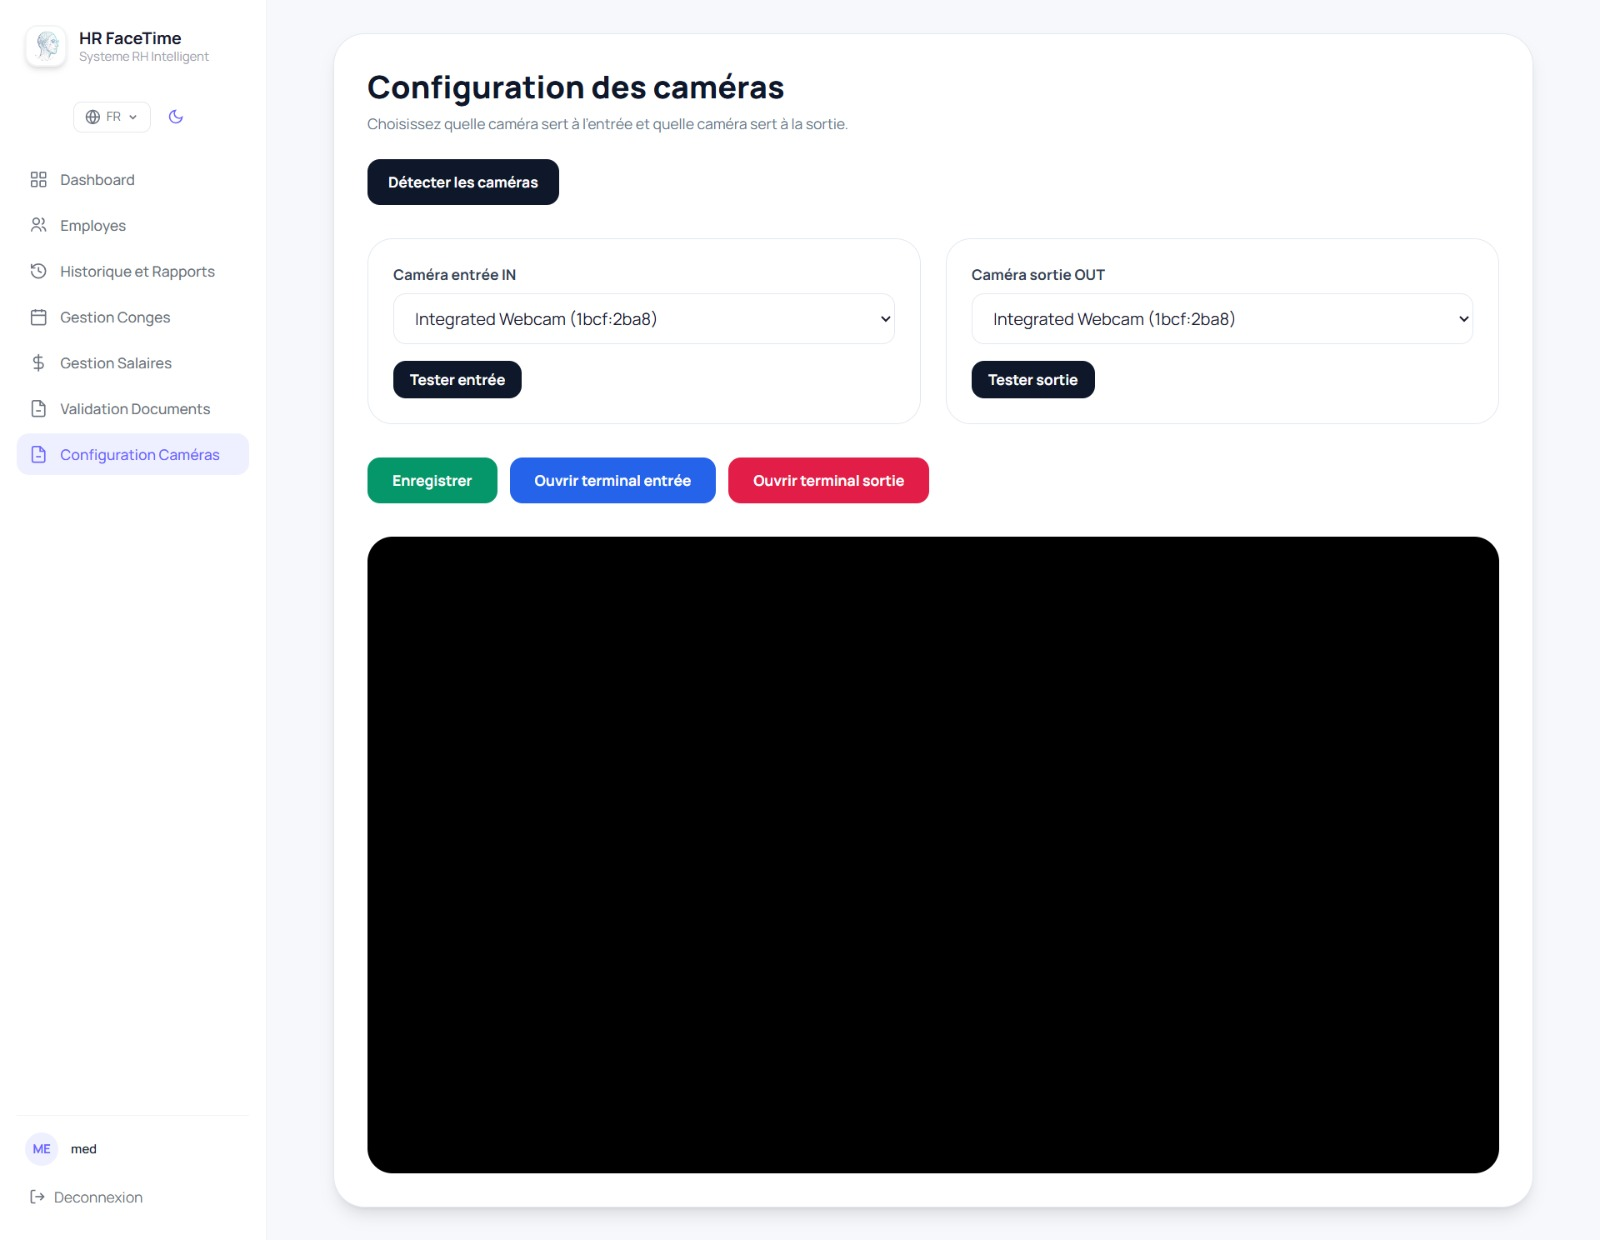
\includegraphics[width=0.9\textwidth]{projet/images/interface/s2/connecter camera.jpeg}
    \caption{Connecter la plateforme aux caméras}
    \label{fig:interface6}
\end{figure}


\subsubsection*{Enregistrer le visage}

Cette interface permet d'enregistrer les données faciales d'un utilisateur pour la reconnaissance et l'identification automatique.

\begin{figure}[H]
    \centering
    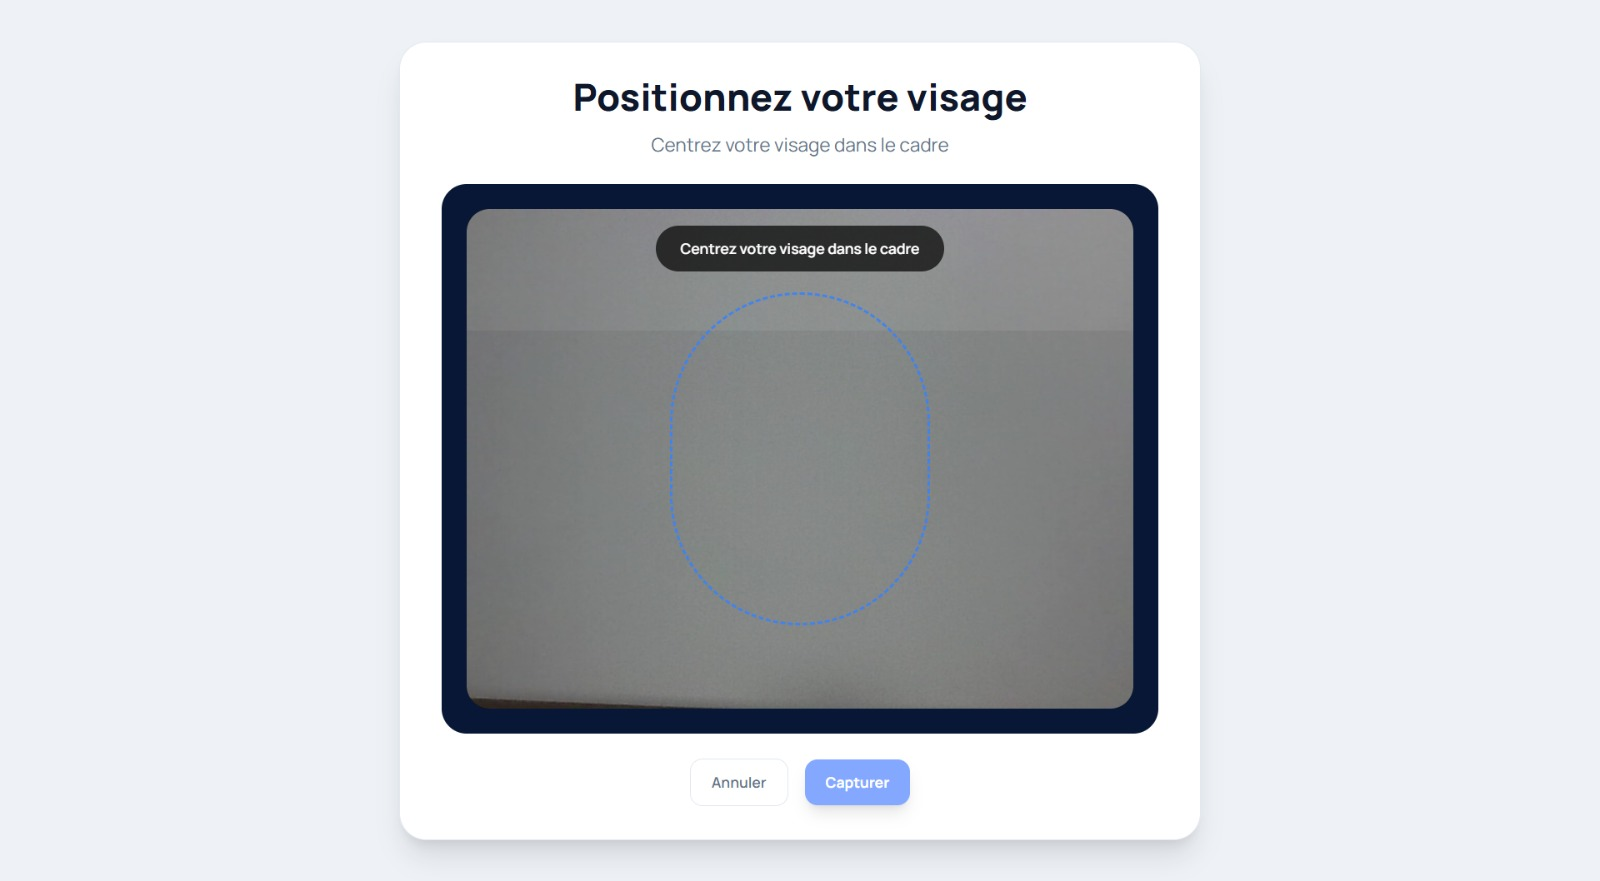
\includegraphics[width=0.9\textwidth]{projet/images/interface/s2/enregister visage.jpeg}
    \caption{Enregistrer le visage}
    \label{fig:interface7}
\end{figure}


\subsubsection*{Modifier infos personnelles}

Cette interface permet à l'utilisateur de modifier ses informations personnelles telles que le nom, l'e-mail ou le mot de passe.

\begin{figure}[H]
    \centering
    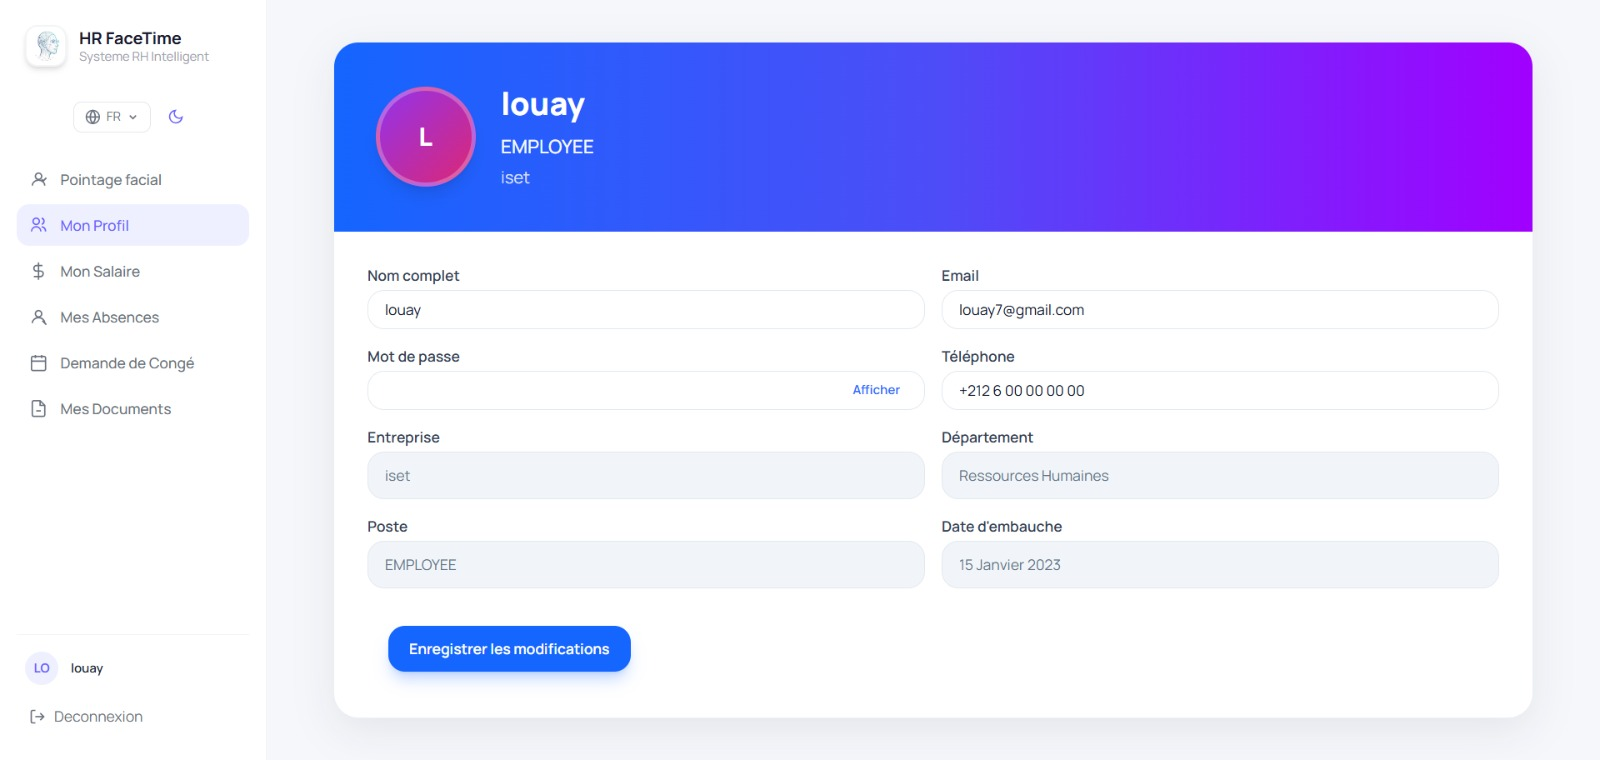
\includegraphics[width=0.9\textwidth]{projet/images/interface/s2/modifier profile.jpeg}
    \caption{Modifier infos personnelles}
    \label{fig:interface8}
\end{figure}


\subsubsection*{Consulter mes absences}

Cette interface permet à l'utilisateur de consulter l'historique et les détails de ses absences enregistrées.

\begin{figure}[H]
    \centering
    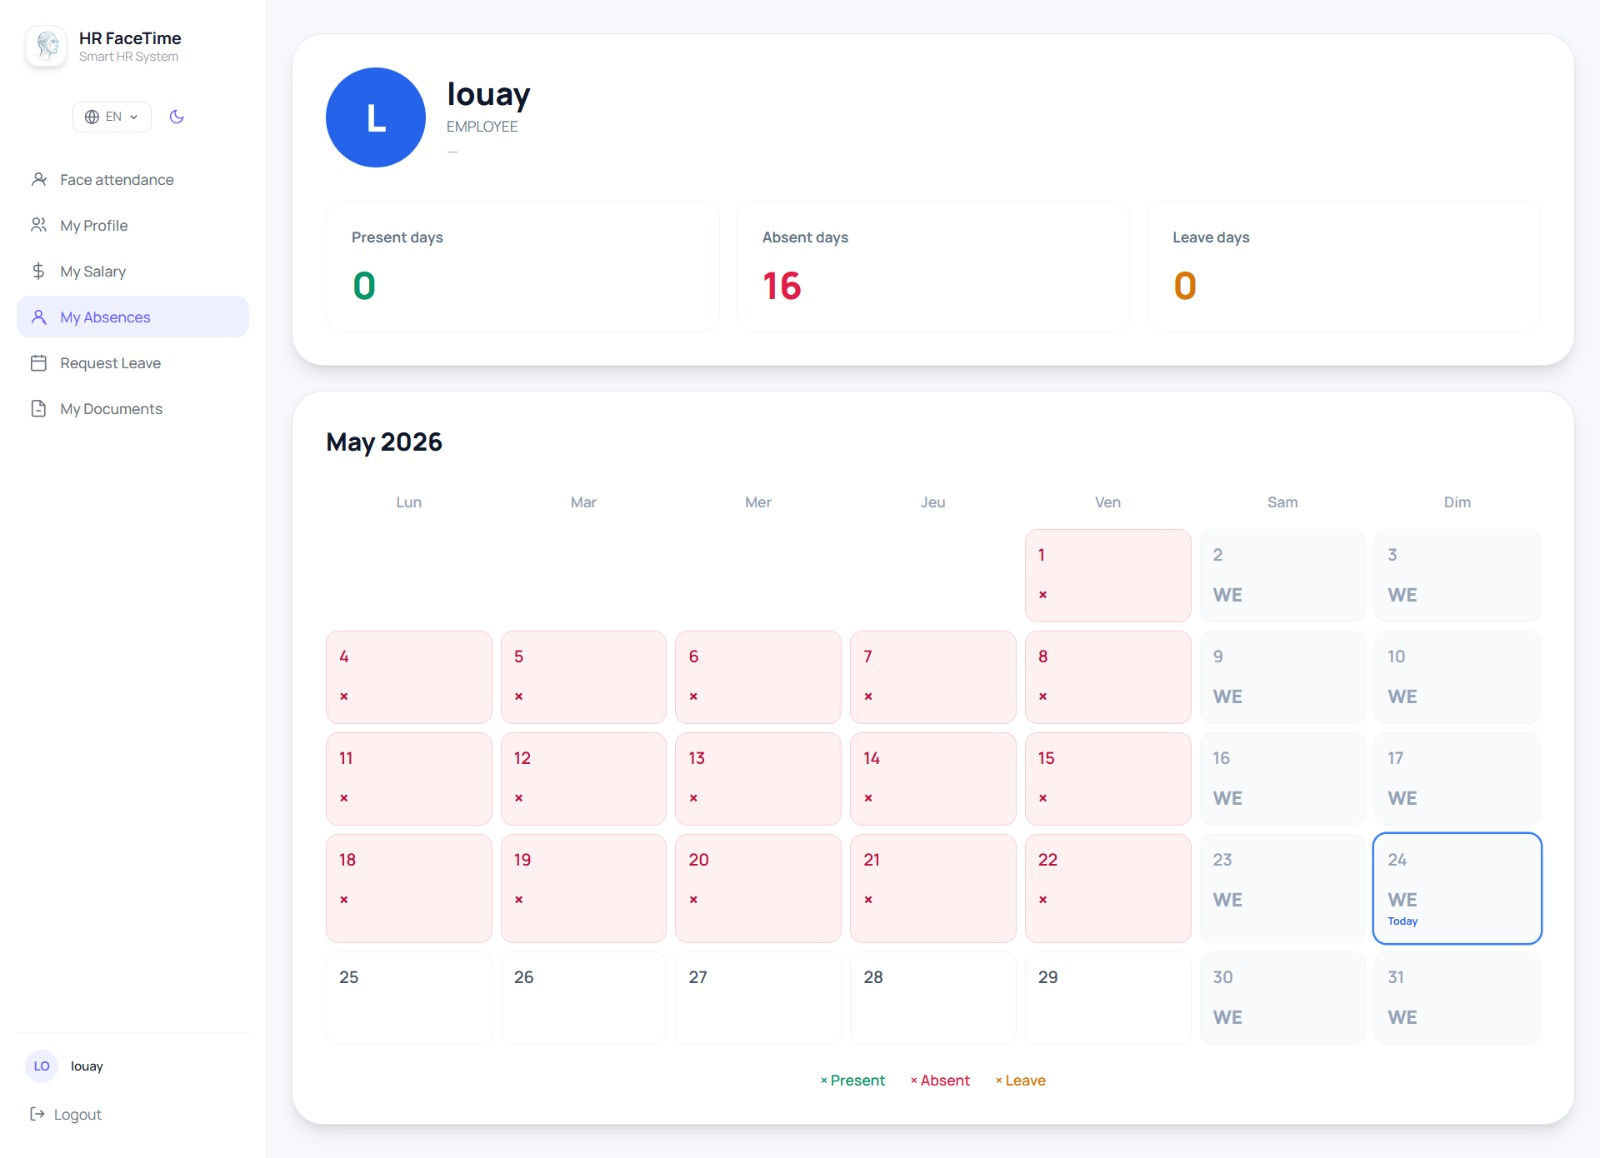
\includegraphics[width=0.9\textwidth]{projet/images/interface/s2/absence.jpeg}
    \caption{Consulter mes absences}
    \label{fig:interface9}
\end{figure}


\subsubsection*{Interface de pointage facial}

L'interface de pointage facial permet aux employés d'enregistrer automatiquement leur présence et leur départ via la reconnaissance faciale.

\begin{figure}[H]
    \centering
    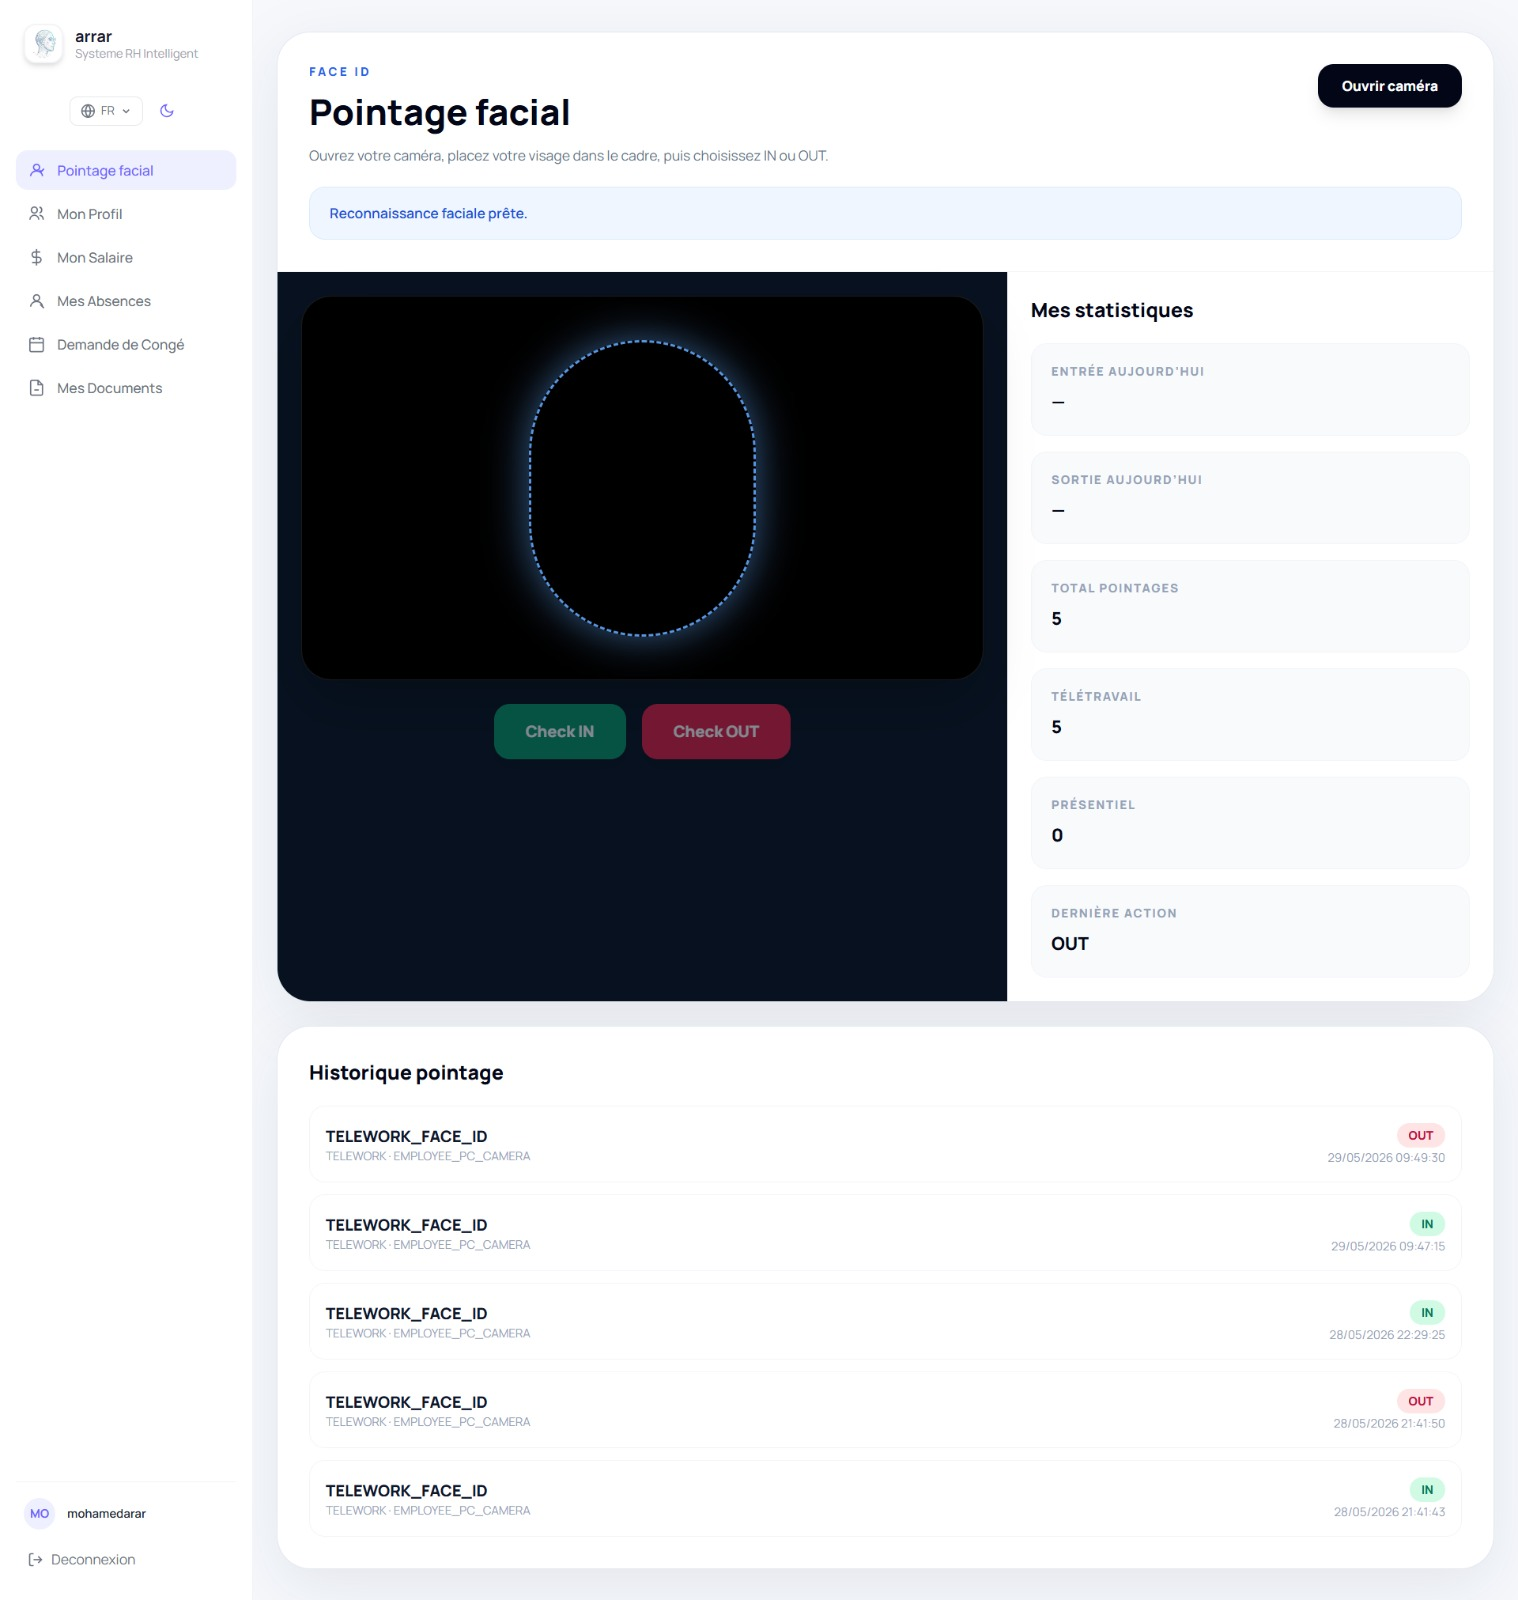
\includegraphics[width=0.9\textwidth]{projet/images/interface/s2/pointage_facial.jpeg}
    \caption{Interface de pointage facial}
    \label{fig:pointage_facial}
\end{figure}


%============================================================
\section{Conclusion}
%============================================================

Cette première release établit les bases essentielles du système en assurant une authentification sécurisée et une gestion efficace des comptes des différents acteurs. Elle intègre également la gestion des employés ainsi qu'un système de pointage intelligent basé sur la reconnaissance faciale, permettant un suivi précis des présences, absences et retards, et offrant au Responsable RH un meilleur contrôle de l'assiduité du personnel.